\documentclass[a4paper, 10pt]{article}
\usepackage[a4paper,margin=1in,bottom=2.5cm,top=2.5cm, headheight=26pt]{geometry}
\geometry{a4paper}
\usepackage{graphicx}
\usepackage{amssymb}
\usepackage[utf8]{inputenc}
\usepackage[brazil]{babel}
\usepackage{color}
\usepackage{float}
\usepackage{hyperref}
\usepackage{fancyhdr}
\usepackage{indentfirst}

\pagestyle{fancy}

\lhead{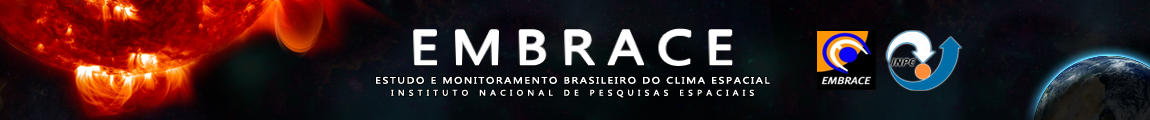
\includegraphics[width=10cm]{embracetopimage.png}}

\title{\Large{\textbf{Briefing Clima Espacial}}}
\date{16/05/2022}

\begin{document}
\maketitle 

  \thispagestyle{fancy} \section{Sol} 
 \subsection{Responsável: José Cecatto}

09/05 – Sem vento rápido; 5 CME p.t.c. para a Terra; \\ 10/05 – 1 flare X1; Sem vento rápido; 6 CME p.t.c. para a Terra; \\ 11/05 – 3 flares M5-; Sem vento rápido; 12 CME p.t.c. para a Terra;  \\ 12/05 – 1 flare M1; Sem vento rápido; 8 CME p.t.c. para a Terra;  \\ 13/05 – Sem vento rápido; 11 CME p.t.c. para a Terra; \\ 14/05 – Sem vento rápido; 2 CME p.t.c. para a Terra; \\ 15/05 – 1 flare M2; Vento solar rápido ($<$ 600 km/s); 1 CME p.t.c. para a Terra; \\ 16/05 – 1 flare M2; Vento solar rápido ($<$= 550 km/s); Sem CME para a Terra; \\ Prev.: Vento solar rápido até 18 de maio; relativamente baixa probabilidade de “flares” (35\% M, 10\% X) nos \\ próximos 02 dias; eventualmente outros CME podem ter componente dirigida para a Terra. \\ p.t.c. – pode(m) ter componente \\ END \\  \\ Thank you !\section{Sol} 
 \subsection{Responsável: Douglas Silva}

\begin{itemize} 
 \item EMC (https://ccmc.gsfc.nasa.gov/donki/):
\item WSA-ENLIL (Ejecoes de Massa Coronal (EMCs) 2022-05-06T17:12Z, 2022-05-06T21:24Z)
\begin{itemize} 
 \item As simulacoes indicam que os flancos das EMCs alcancarao a missao DSCOVR entre 2022-05-11T04:00Z e 2022-05-11T18:00Z.
\end{itemize} 
 \item WSA-ENLIL (Ejecoes de Massa Coronal (EMCs) :2022-05-10T15:12Z e 2022-05-10T14:48Z)
\begin{itemize} 
 \item Os resultados das simulacoes indicam que as bordas frontais combinada das EMCs alcancara a missao DSCOVR entre 2022-05-13T16:00Z e 2022-05-14T06:00Z.
\end{itemize} 
 \item WSA-ENLIL (Ejecao de Massa Coronal (EMC) :2022-05-10T14:48Z)
\begin{itemize} 
 \item Os resultados das simulacoes indicam que o flanco da EMC alcancara a missao DSCOVR entre 2022-05-13T21:00Z e 2022-05-14T11:00Z 
\end{itemize} 
 \end{itemize} 
 

    \begin{figure}[H]
        \centering
        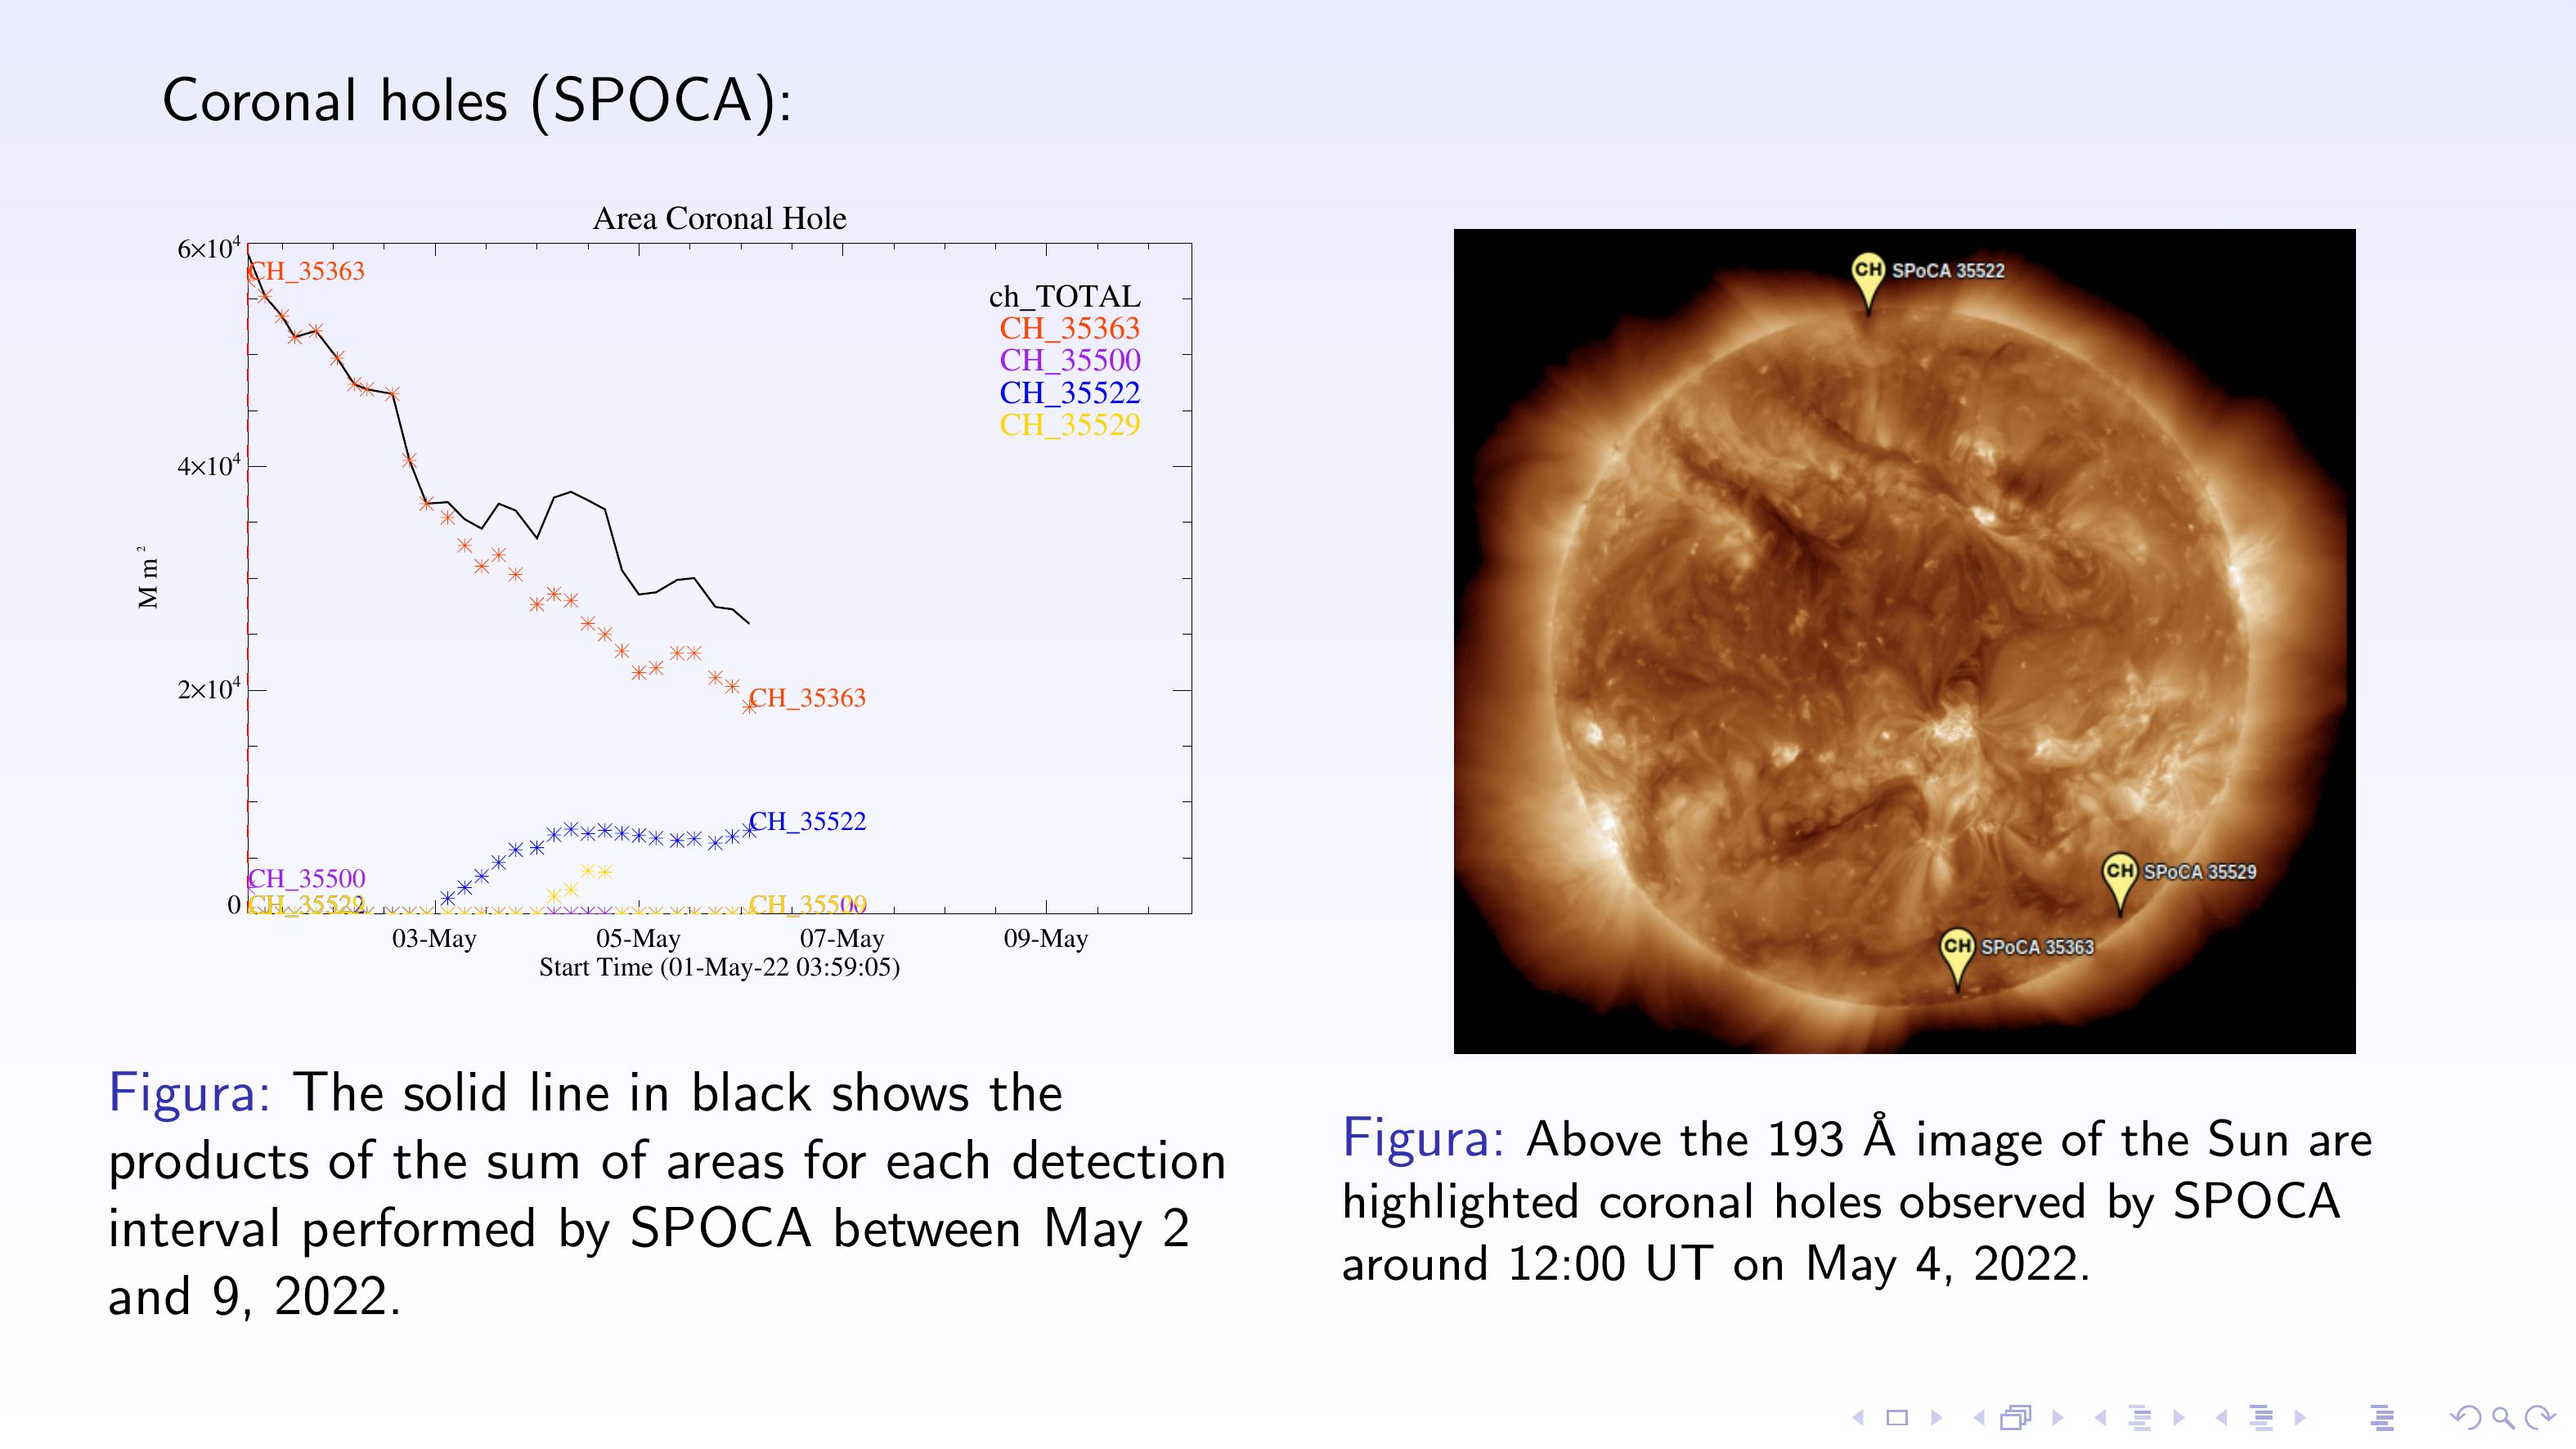
\includegraphics[width=14cm]{./figures/pt_outfileSun_0.jpg}
    \end{figure} 
 

    
    \begin{figure}[H]
        \centering
        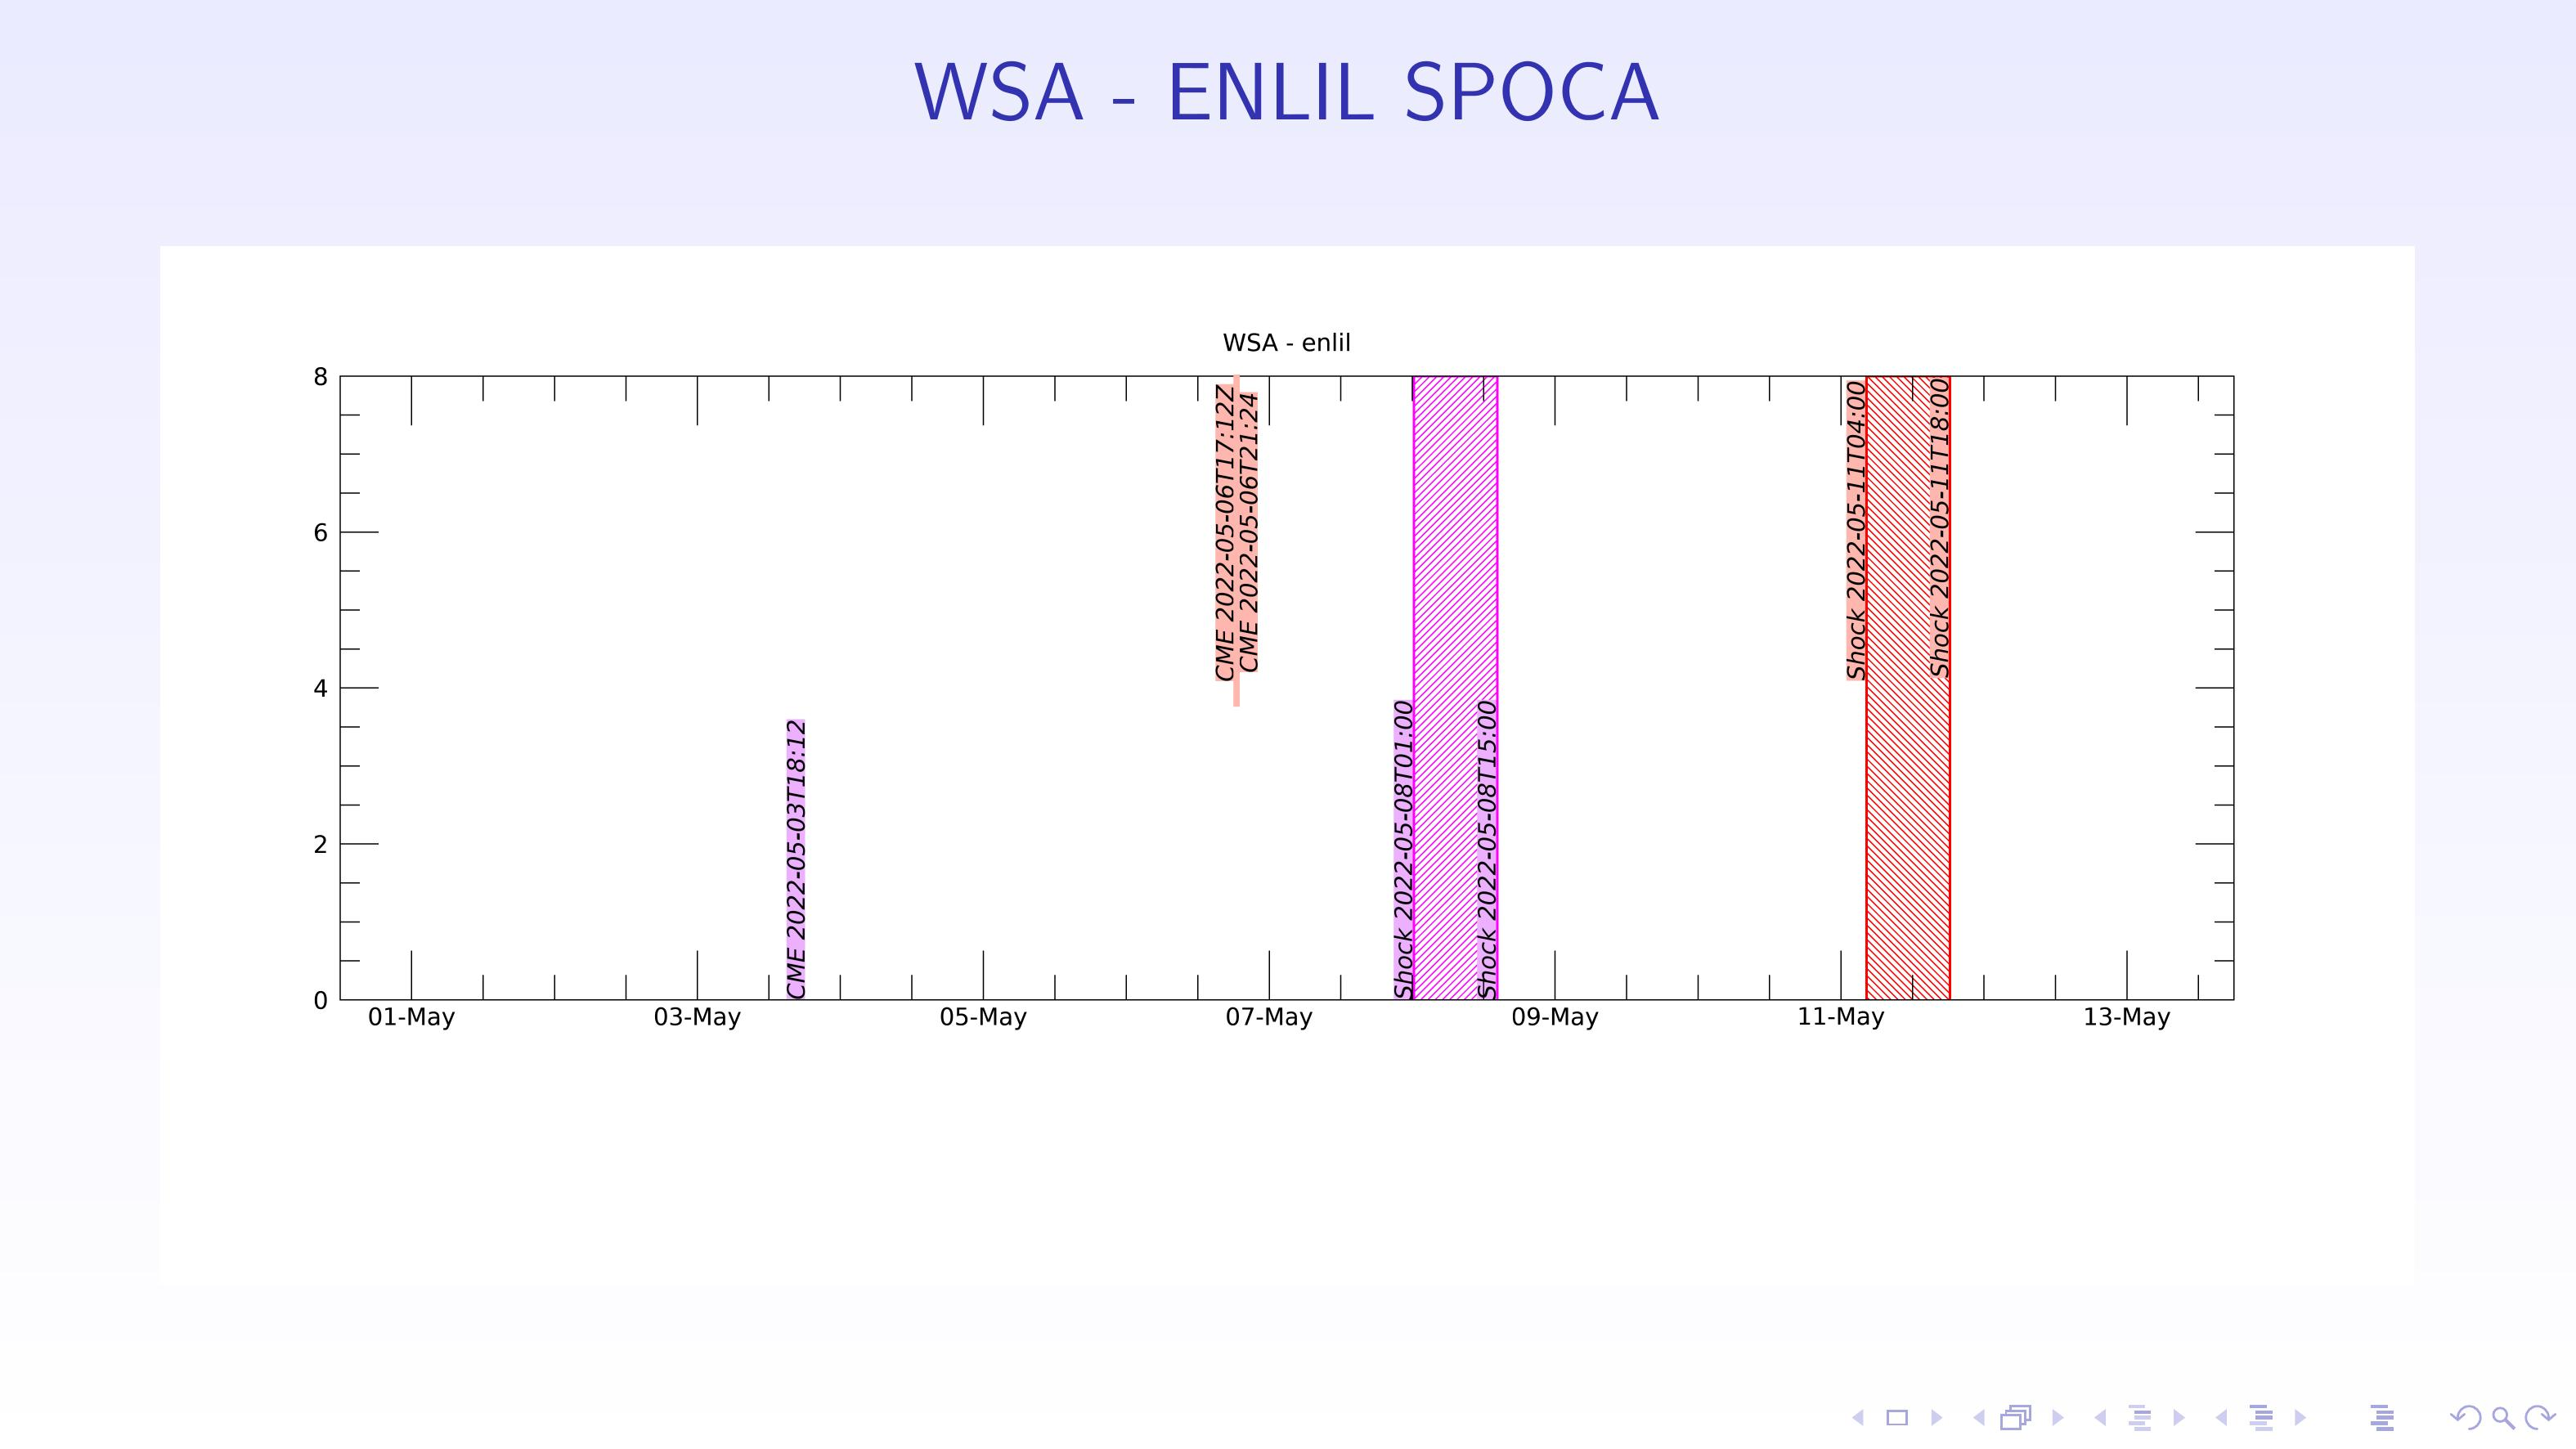
\includegraphics[width=14cm]{./figures/pt_outfileSun_1.jpg}
    \end{figure} 
 

    \section{Meio Interplanetário} 
 \subsection{Responsável: Paulo Jauer} 
 
 \begin{figure}[H]
    \centering
    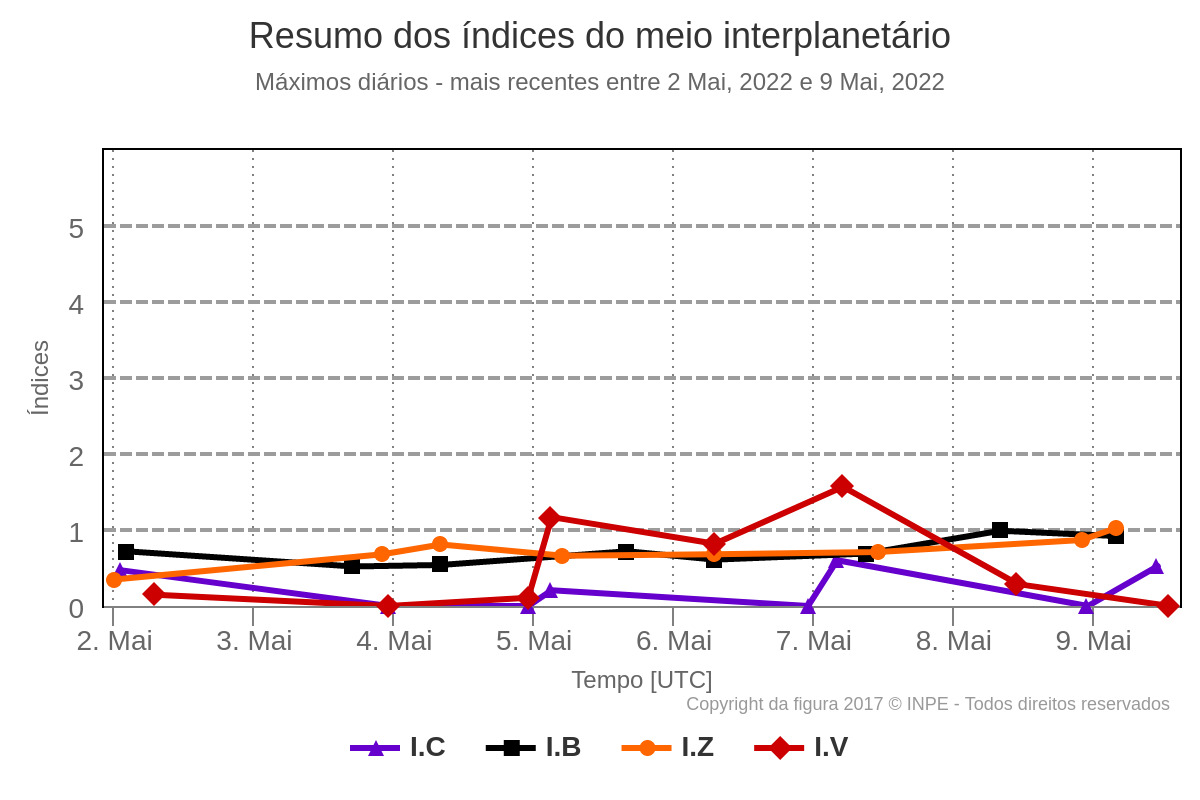
\includegraphics[width=14cm]{./figures//figureMIIndex.png}
\end{figure}
 \begin{itemize}
 \item A região do meio interplanetário na última  semana apresentou um nível  baixo a moderado nas perturbações  do plasma devido à possível interação de estruturas do tipo CME e HSS identificadas pelo satélite DISCOVERY no meio interplanetário.
\item O modulo da componente do campo magnético interplanetário apresentou 1 pico máximo : 14/Mai às 18:30  de ~ 18 nT. 
\item As componentes BxBy apresentaram variações no período analisado, mantendo-se ambas oscilando dentro do intervalo [+10, -10] nT, com troca de setor no dia 12 de maio às 13:30.  
\item A componente do campo bz apresentou flutuações com valor positivo de de 12 nT no dia 16/Maio às 02:30 e valor negativo de -9.19 nT às 19:30 UT no dia 11/Maio.  Na média  a componente Bz  oscilou majoritariamente negativa. Condições favoráveis ao surgimento de perturbações geomagnéticas.
\item A densidade do vento solar oscilou majoritariamente abaixo de 10 p/cm³ durante o período analisado com pico máximo no dia 012/Maio às 13:30 de 23 p/cm³, e outro pico no dia 14 de maio às 17:30 de 27 p/cm³. 
\item A velocidade do vento solar teve oscilando majoritariamente abaixo de 400 km/s até o dia 14 de maio às 20:30 mudando para valores maiores com pico no dia 15 de maio às de 566 km/s.
\item A posição da magnetopausa esteve oscilando em média  na posição tipica 10 Re. Apresentou duas compressão significativa no dia 14 e 15 de maio de 8.6 Re às 17:30 e 03:30 UT respectivamente.
\item   
\item  
\end{itemize} 
\section{Cinturões de Radiação} 
 \subsection{Responsável: Ligia Alves da Silva} 
 
\begin{figure}[H]
    
                        \centering
   
                             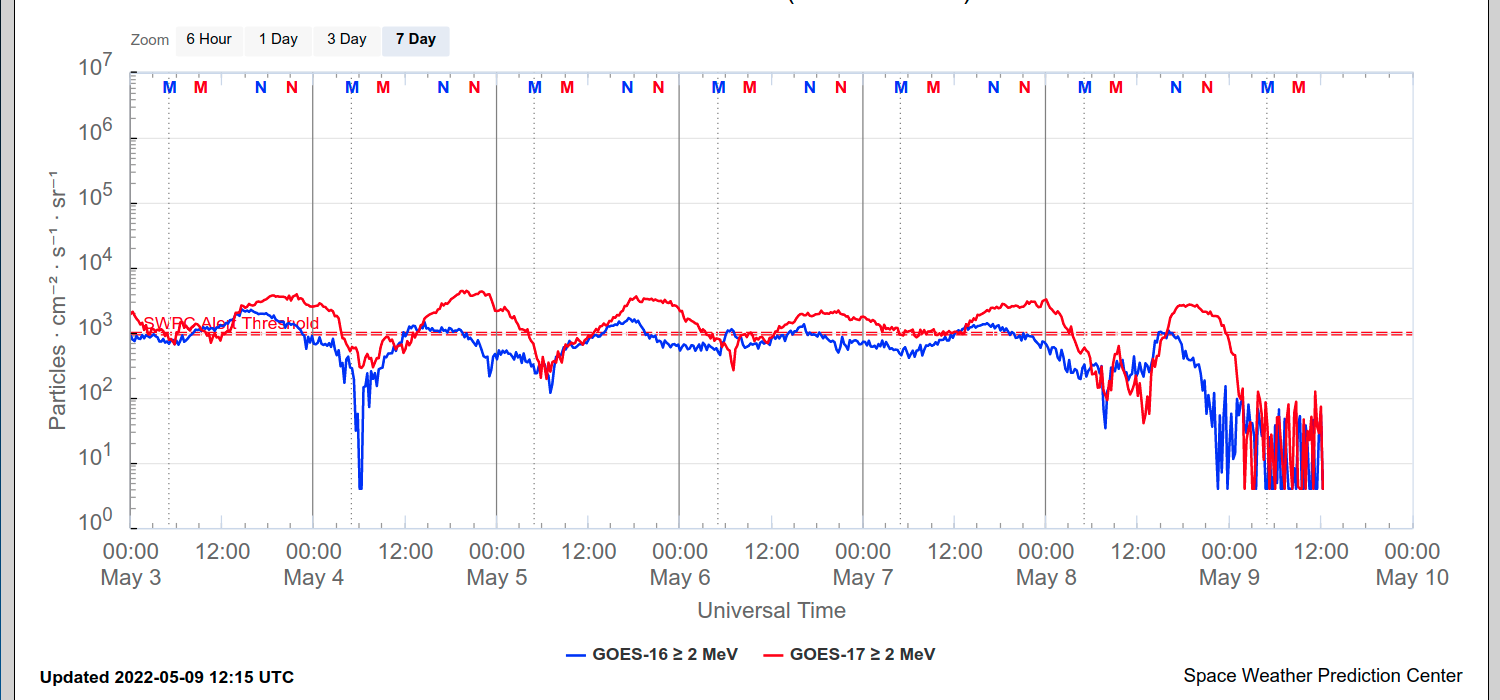
\includegraphics[width=14cm]{./figures//figureRadBelts_0.png}

                             \caption{ Fluxo de elétrons de alta energia (> 2MeV) obtido a partir dos satélites GOES-16 e GOES-17. Fonte}
                        \end{figure}

                     \begin{figure}[H]
    
                        \centering
   
                             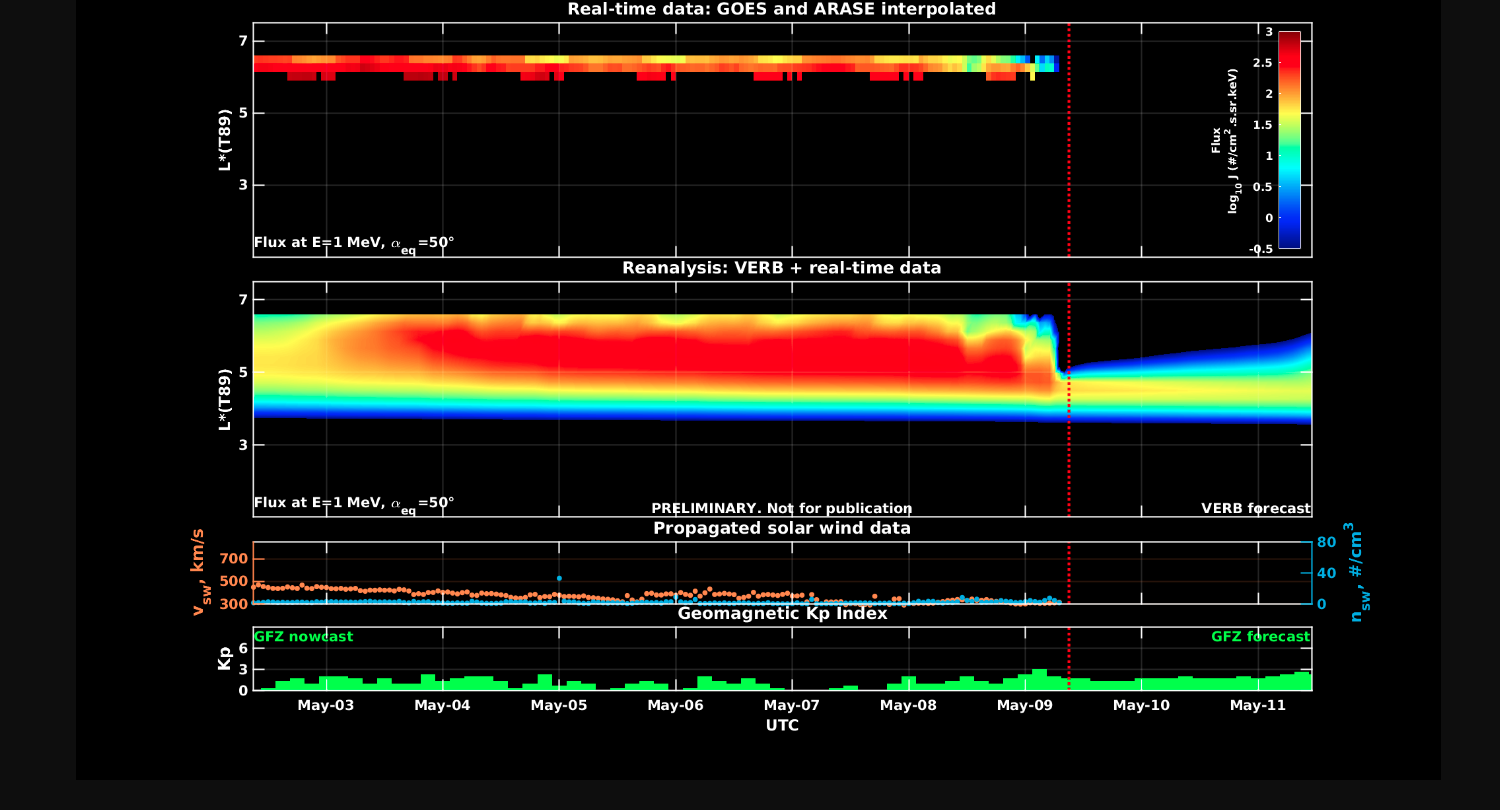
\includegraphics[width=14cm]{./figures//figureRadBelts_1.png}

                             \caption{ Dados de fluxo de elétrons de alta energia (reais e interpolados) obtidos a partir dos satélites ARASE, GOES-16, GOES-17. Dados reanalisados a partir do VERB code e do fluxo de elétrons interpolados. Dados da velocidade do vento solar e densidade de prótons obtidos a partir do satélite ACE. Fonte}
                        \end{figure}

                     O fluxo de Elétrons de alta energia (>2 MeV) na borda do cinturão de radiação externo obtidos a partir do satélite geoestacionário GOES-16 e GOES-17 (Figura 1) apresenta-se abaixo de 102 partículas/(cm2 s sr) durante toda a semana de analise. Observa-se uma diminuição de fluxo de elétrons significativa no início do dia 12 de maio, retirando quase que completamente a população de elétrons de alta energia da borda do cinturão externo de radiação. A partir das 12:00 UT a borda retorna aos valores iniciais de 102 partículas/(cm2 s sr). 

Os dados dos satélites ARASE, GOES-16 e GOES-17 são analisados e interpolados para que a variabilidade do fluxo de elétrons de alta energia (1 MeV) seja observada em todo o cinturão externo de radiação (Figura 2). Adicionalmente o VERB code reconstrói este fluxo considerando a difusão radial por ondas Ultra Low Frequency (ULF). A simulação (VERB code) mostra que a diminuição de fluxo de elétrons atingiu L-shell > 5.0. A partir das 12:00 UT do dia 15 de maio observa-se um aumento de fluxo de elétrons entre 4.5 < L-shell < 5.5. Estas variabilidades no fluxo de elétrons ocorreram concomitantes a chegada de estruturas do vento solar e atividades de ondas ULF. Contudo, é importante salientar que os dados do satélite ARASE não estão disponíveis para a semana em análise, para confirmação do nível de L-shell destas variabilidades no fluxo de elétrons.



\section{Ondas ULF} 
 \subsection{Responsável: José Paulo Marchezi} 
 
\begin{figure}[H]
    
                        \centering
   
                             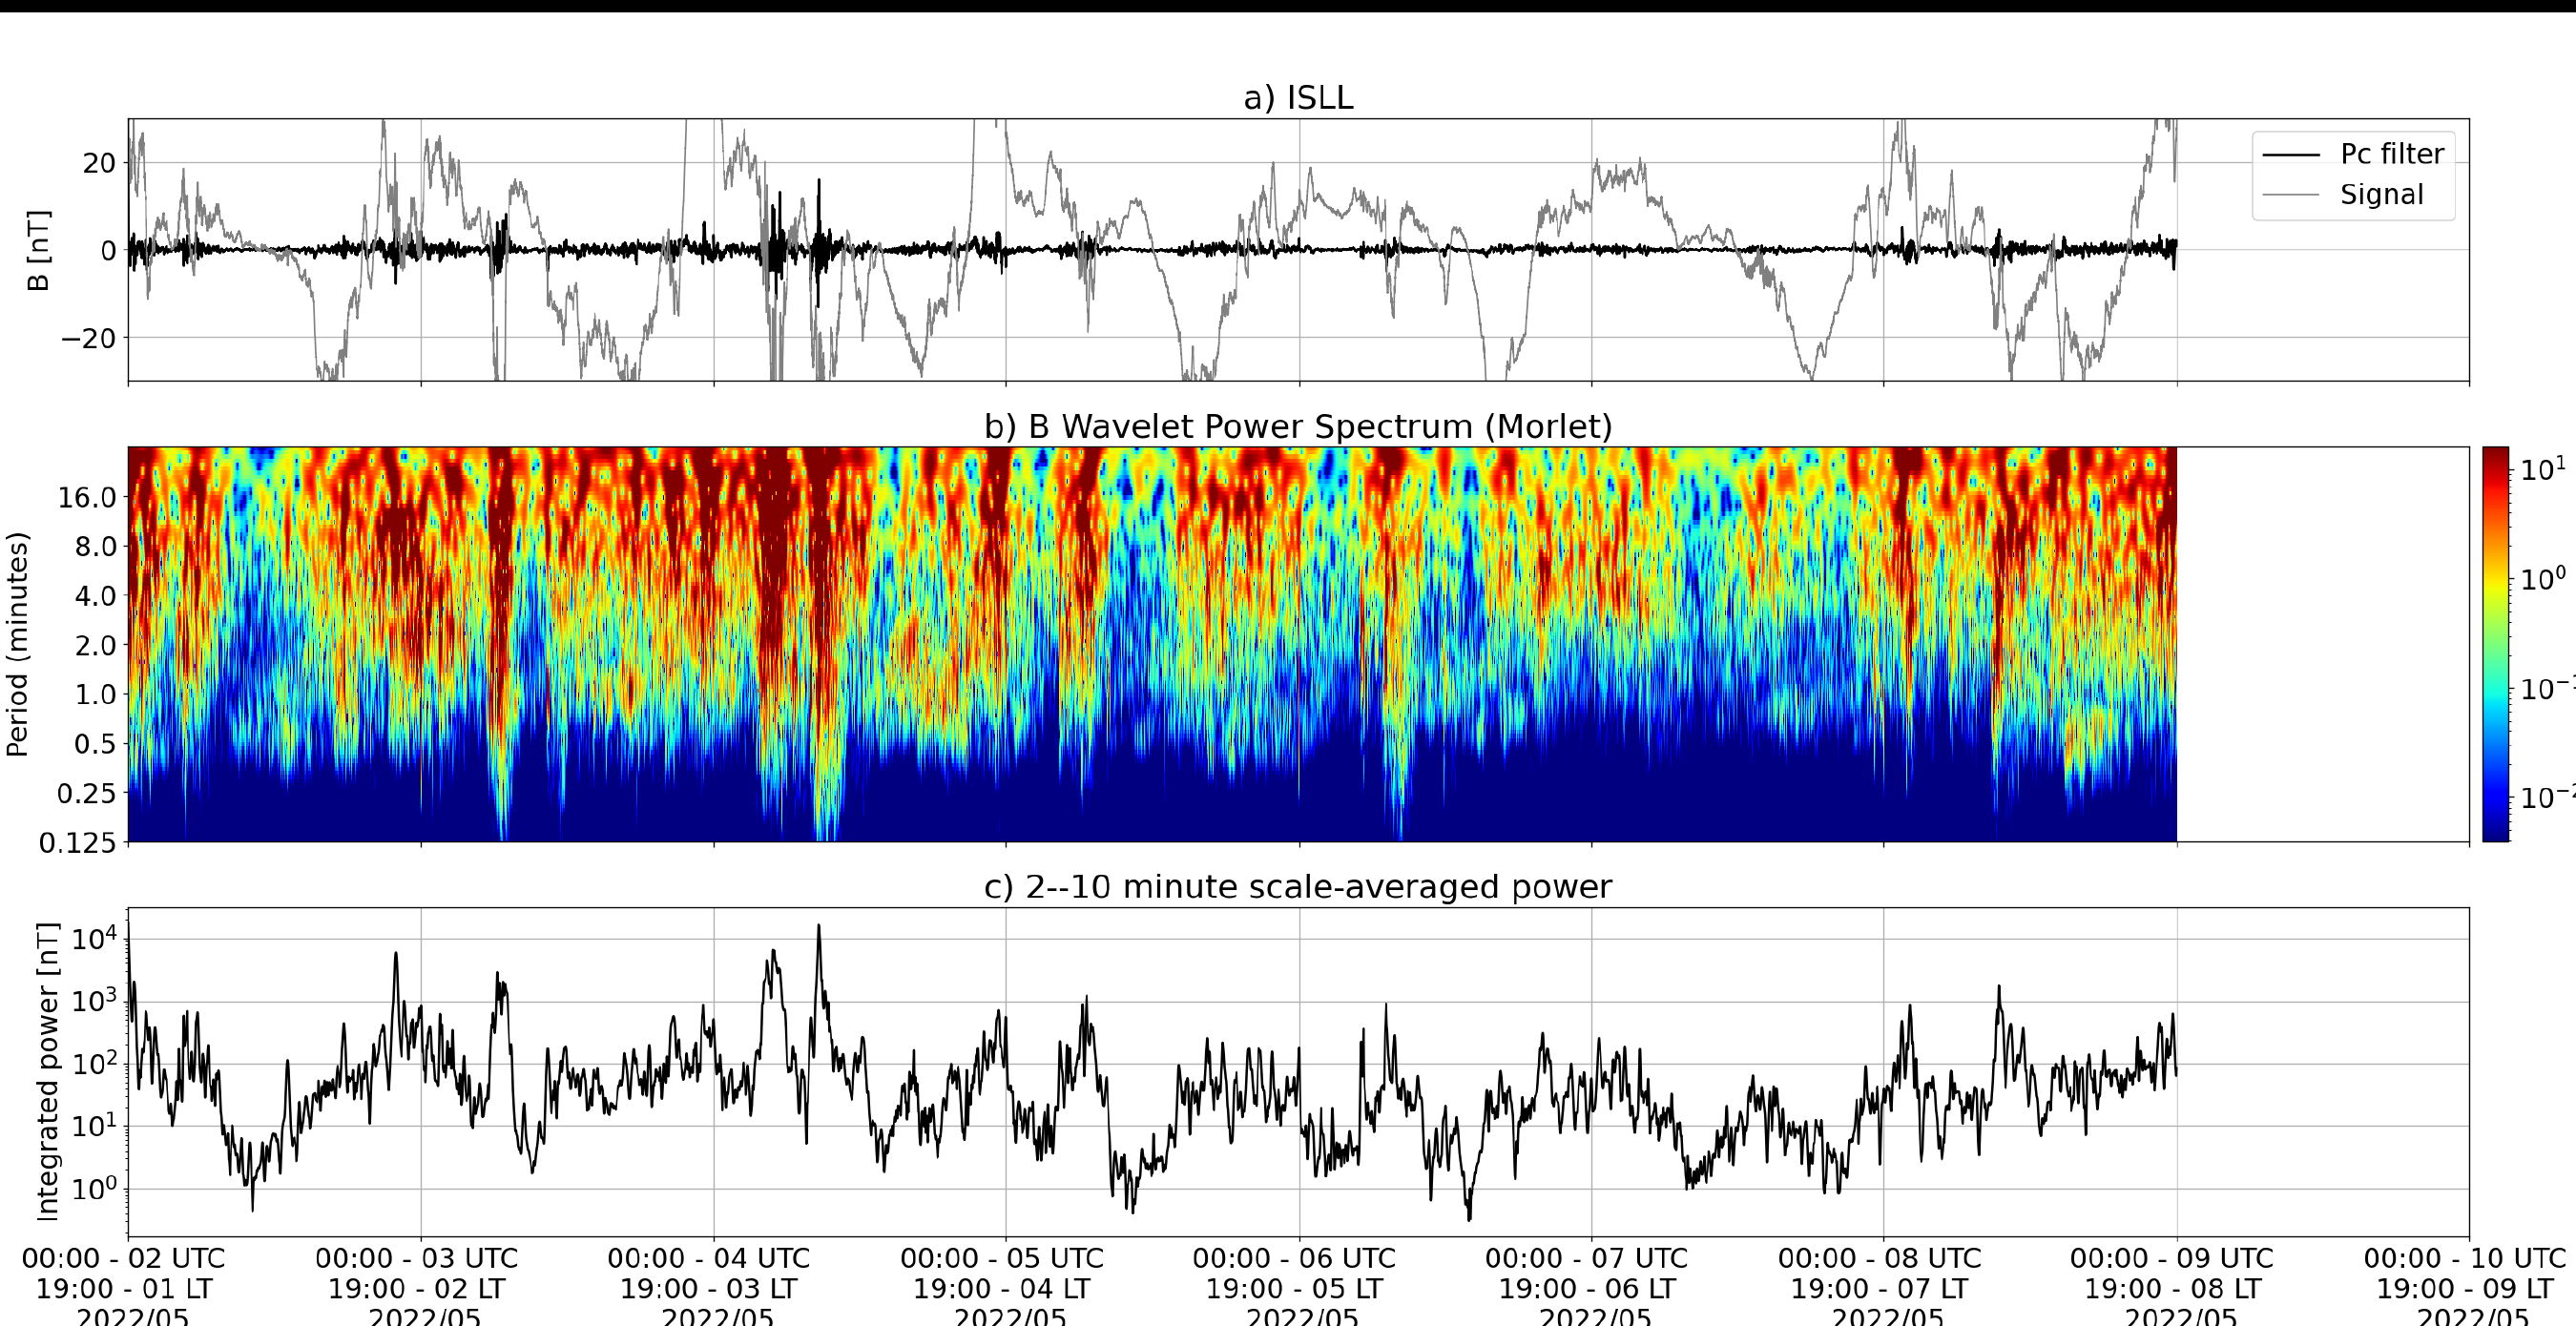
\includegraphics[width=14cm]{./figures//figureULF_0.png}

                             \caption{a) sinal do campo magnético total 
                              medido na Estação ISLL da rede CARISMA em cinza, 
                              junto com a flutuação na faixa de Pc5 em preto. b) 
                              Espectro de potência wavelet do sinal filtrado. c) 
                              Média da potência espectral nas faixas de 2 a 10 minutos 
                              (ondas ULF).}
                        \end{figure}

                     \begin{figure}[H]
    
                        \centering
   
                             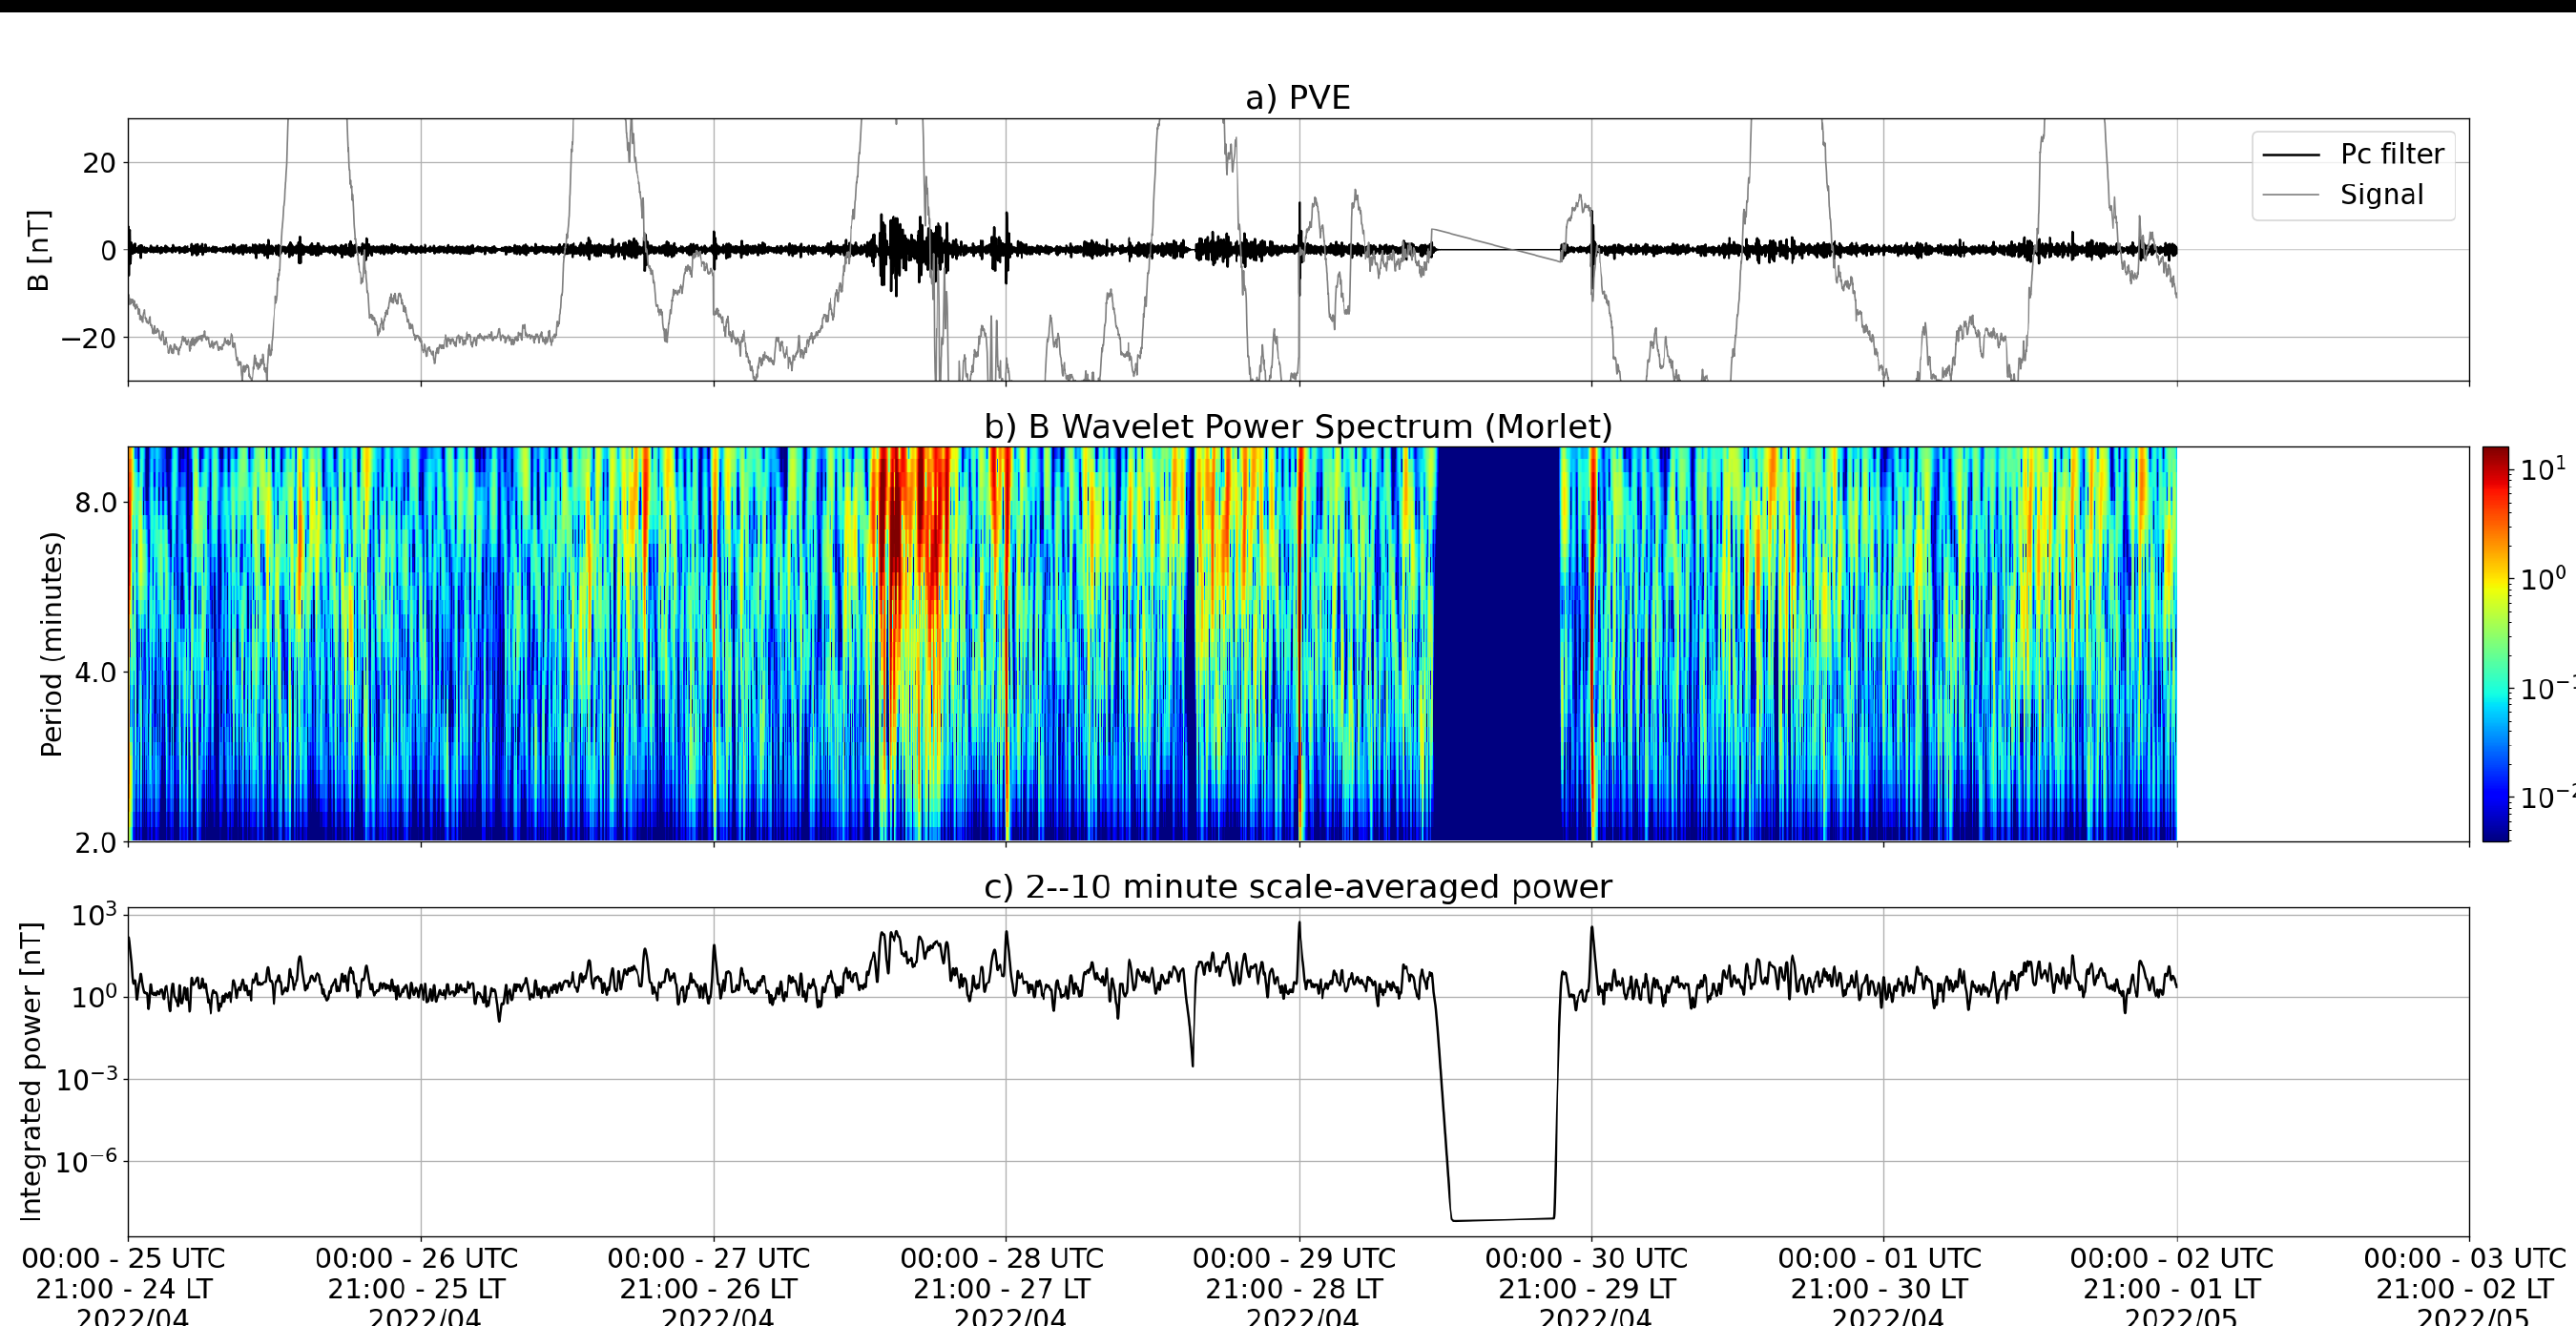
\includegraphics[width=14cm]{./figures//figureULF_1.png}

                             \caption{a) sinal do campo magnético total medido 
                              na Estação SMS da rede EMBRACE em cinza, junto com a 
                              flutuação na faixa de Pc5 em preto. b) Espectro de potência 
                              wavelet do sinal filtrado. c) Média da potência espectral nas 
                              faixas de 2 a 10 minutos (ondas ULF).}
                        \end{figure}

                     \begin{figure}[H]
    
                        \centering
   
                             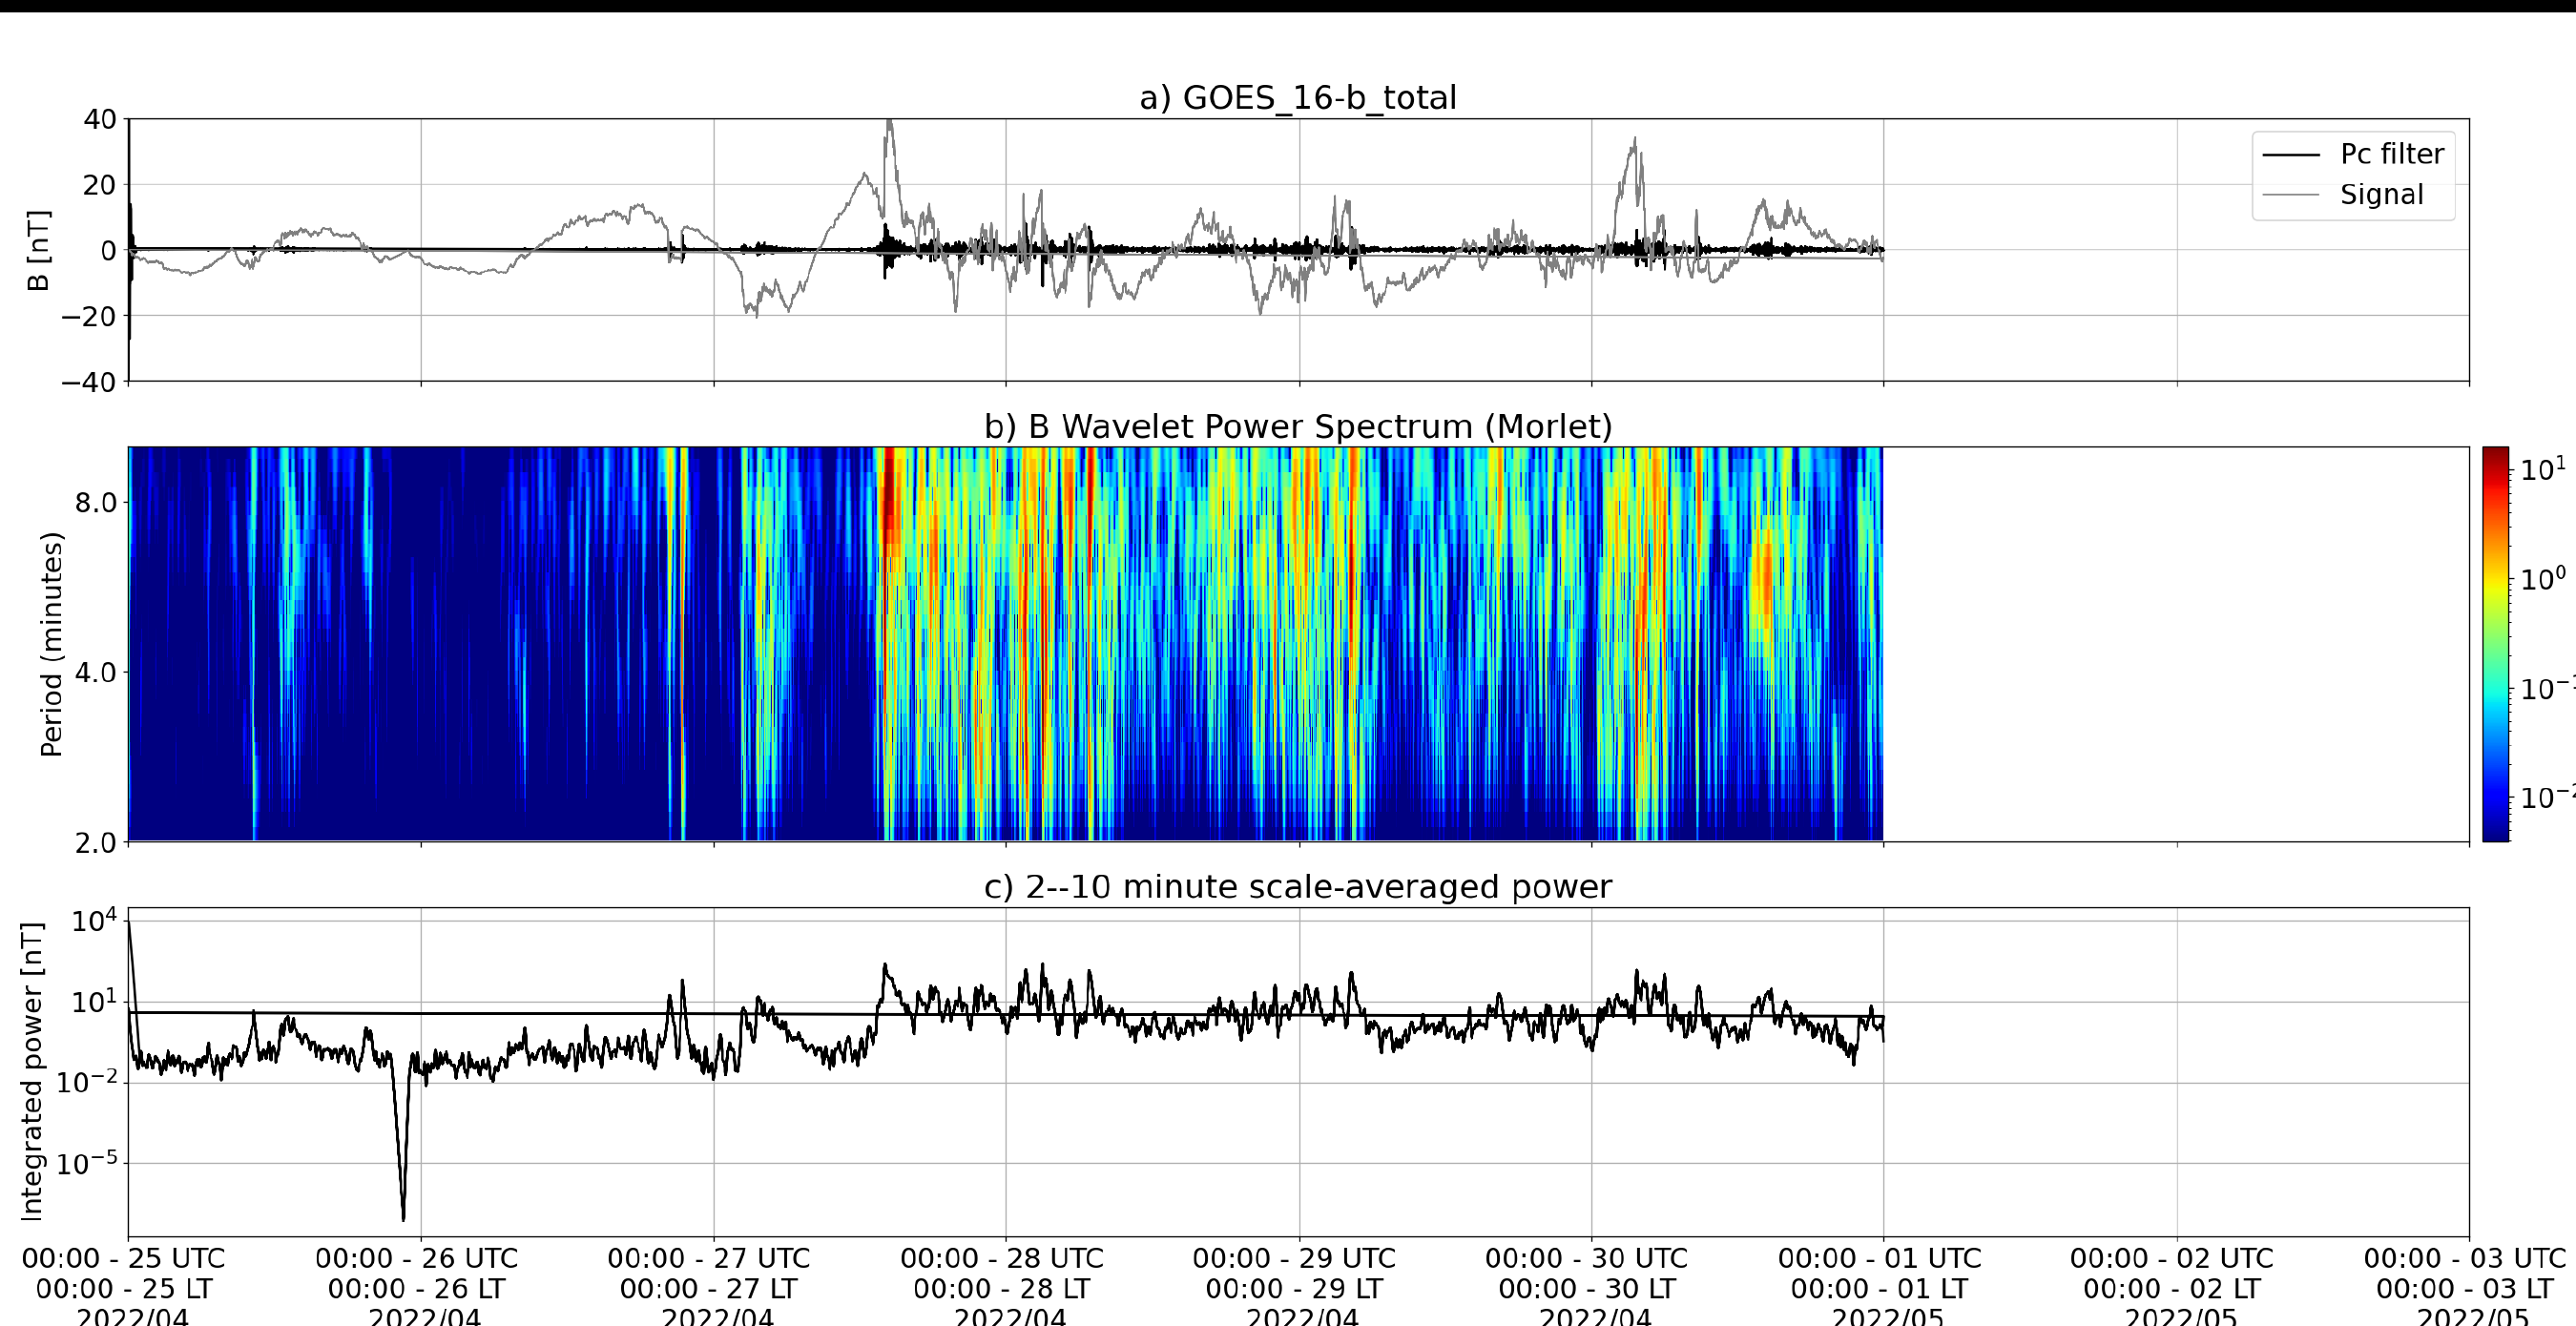
\includegraphics[width=14cm]{./figures//figureULF_2.png}

                             \caption{a) sinal do campo magnético total medido pelo 
                              satélite GOES 16, junto com a flutuação na faixa de Pc5 
                              em preto. b) Espectro de potência wavelet do sinal 
                              filtrado. c) Média da potência espectral nas faixas 
                              de 2 a 10 minutos (ondas ULF).}
                        \end{figure}

                     m No dia 9 de maio há um aumento da potência das ondas ULF com
duração de cerca de 12h, com características contínuas. A atividade de
ondas ULF diminui nos das 10 e 11, e só volta a aumentar na primeira
metade do dia 12, com oscilações de curta duração, cobrindo a faixa de
frequências das pulsações geomagnéticas Pc3-Pc5. Os dados da estação de
Porto Velho (PVE) apresentam bastante flutuações durante todo o período,
possivelmente devido a características locais, sub influência do eletrojato
equatorial. Em São Martinho da Serra há um aumento da potência a partir
do dia 14, característico de uma interação com um choque interplanetário,
seguido de um possível High-Speed Stream. A componente y do campo
magnético medido pelo satélite GOES é a que apresenta maior potência de
ondas, nos dias 9, 12 e 14 de maio.
Sumário
9/10
m No dia 9 de maio há um aumento da potência das ondas ULF com duração de cerca de 12h, com características contínuas. A atividade de ondas ULF diminui nos das 10 e 11, e só volta a aumentar na primeira metade do dia 12, com oscilações de curta duração, cobrindo a faixa de frequências das pulsações geomagnéticas Pc3-Pc5. Os dados da estação de Porto Velho (PVE) apresentam bastante flutuações durante todo o período, possivelmente devido a características locais, sub influência do eletrojato equatorial. Em São Martinho da Serra há um aumento da potência a partir do dia 14, característico de uma interação com um choque interplanetário, seguido de um possível High-Speed Stream. A componente y do campo magnético medido pelo satélite GOES é a que apresenta maior potência de ondas, nos dias 9, 12 e 14 de maio.\section{Ondas EMIC} 
 \subsection{Responsável: Claudia Medeiros} 
 
\begin{figure}[H]
    
                        \centering
   
                             \includegraphics[width=14cm]{./figures//figureEMIC_1.png}

                        \end{figure}

                     \begin{figure}[H]
    
                        \centering
   
                             \includegraphics[width=14cm]{./figures//figureEMIC_2.png}

                        \end{figure}

                     \section{Geomagnetismo} 
 \subsection{Responsável: Livia Riveiro Alves} 
 
\begin{figure}[H]
    
                        \centering
   
                             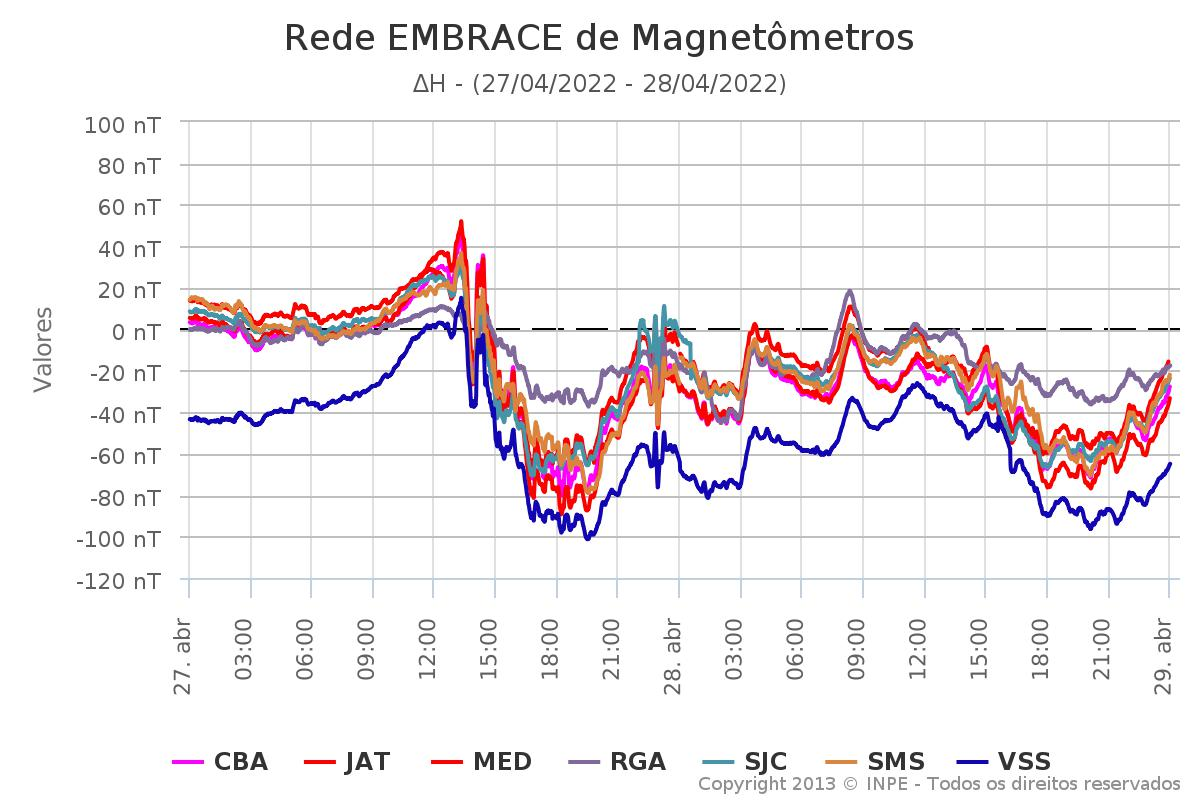
\includegraphics[width=14cm]{./figures//figureGeomag_0.png}

                        \end{figure}

                     \begin{figure}[H]
    
                        \centering
   
                             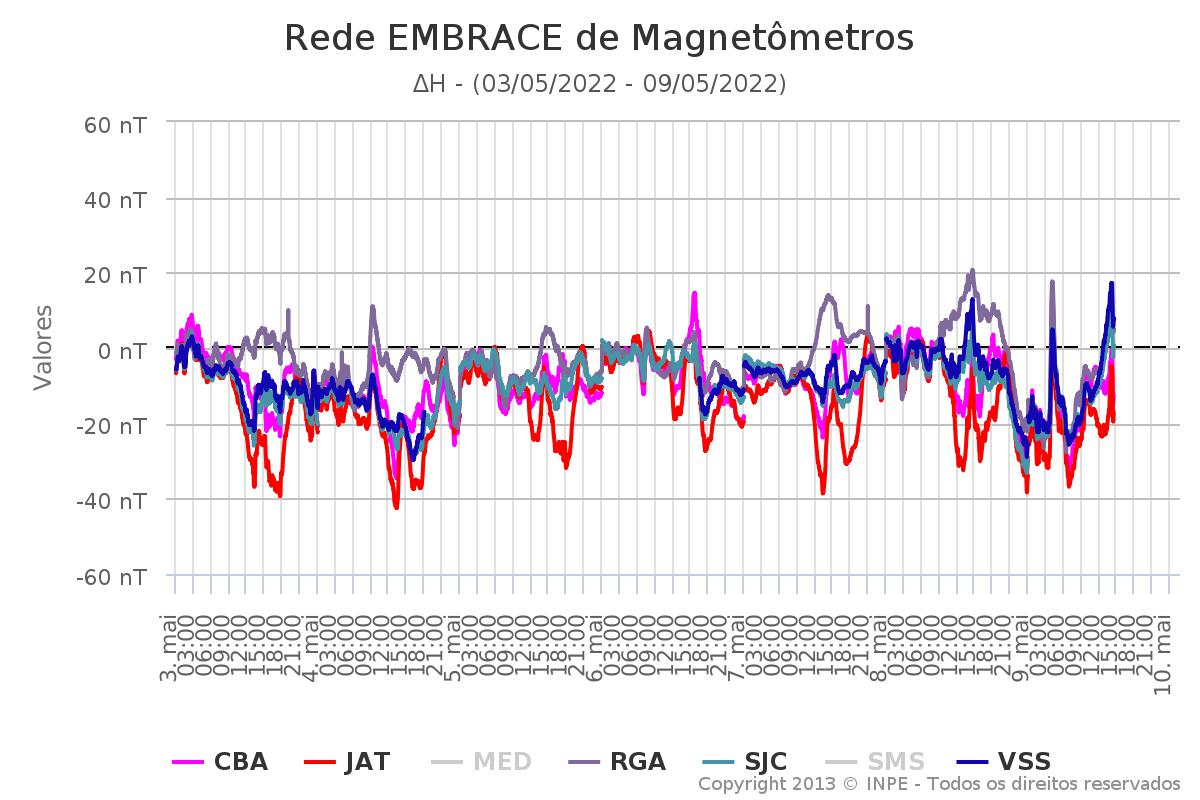
\includegraphics[width=14cm]{./figures//figureGeomag_1.png}

                        \end{figure}

                     \begin{figure}[H]
    
                        \centering
   
                             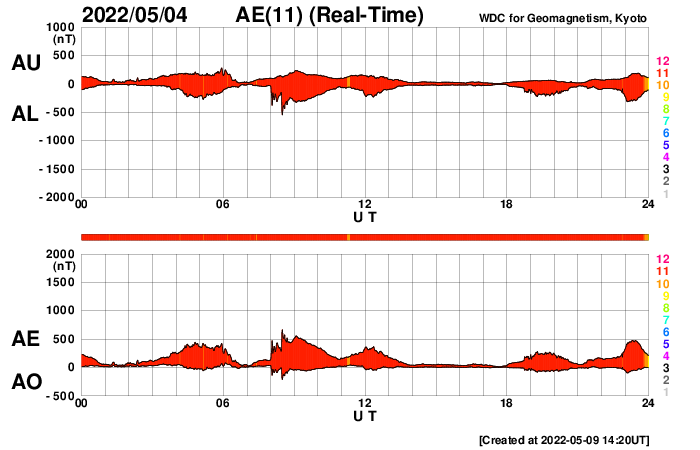
\includegraphics[width=14cm]{./figures//figureGeomag_2.png}

                        \end{figure}

                     \begin{figure}[H]
    
                        \centering
   
                             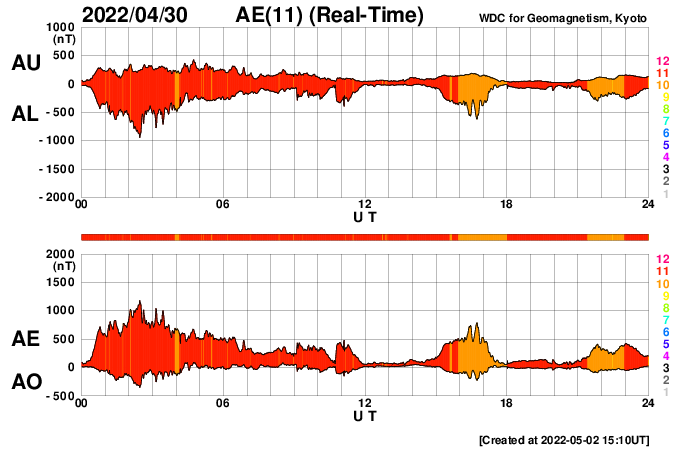
\includegraphics[width=14cm]{./figures//figureGeomag_3.png}

                        \end{figure}

                     \begin{figure}[H]
    
                        \centering
   
                             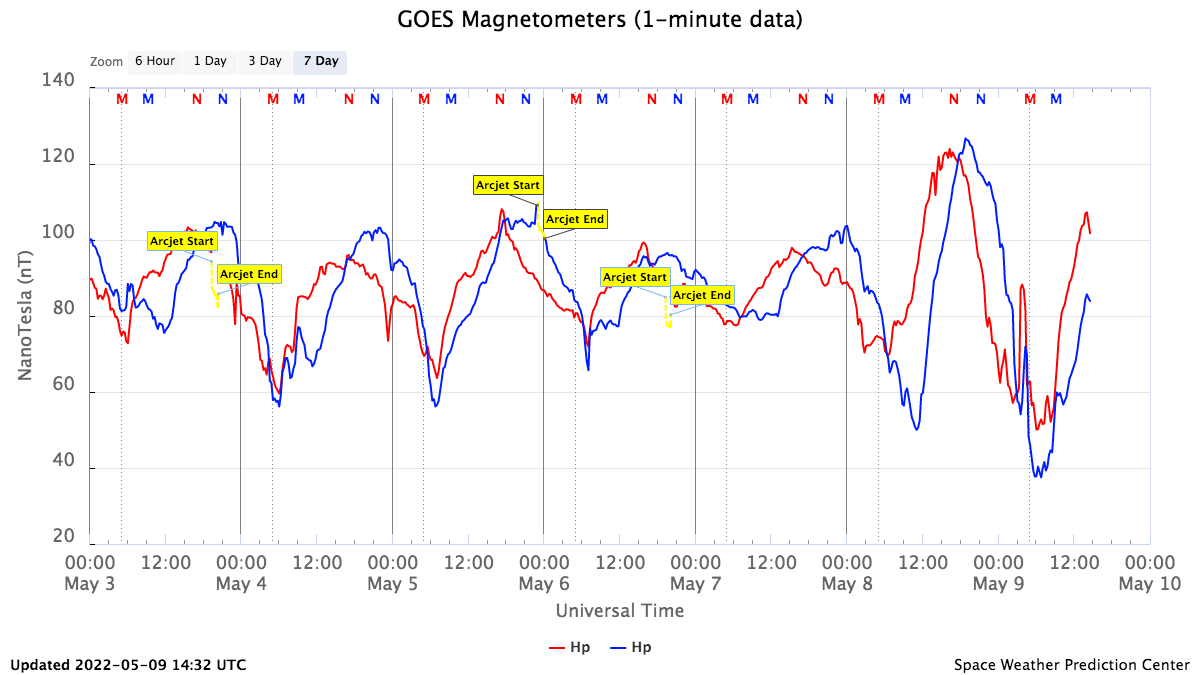
\includegraphics[width=14cm]{./figures//figureGeomag_4.png}

                        \end{figure}

                     \begin{figure}[H]
    
                        \centering
   
                             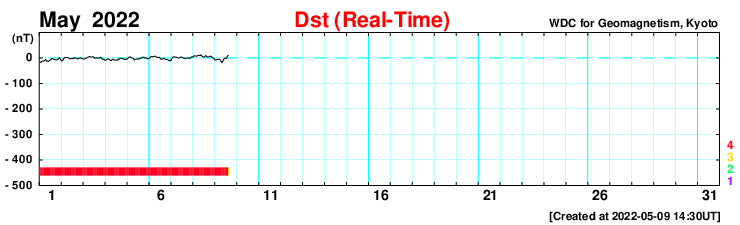
\includegraphics[width=14cm]{./figures//figureGeomag_5.png}

                        \end{figure}

                     \begin{figure}[H]
    
                        \centering
   
                             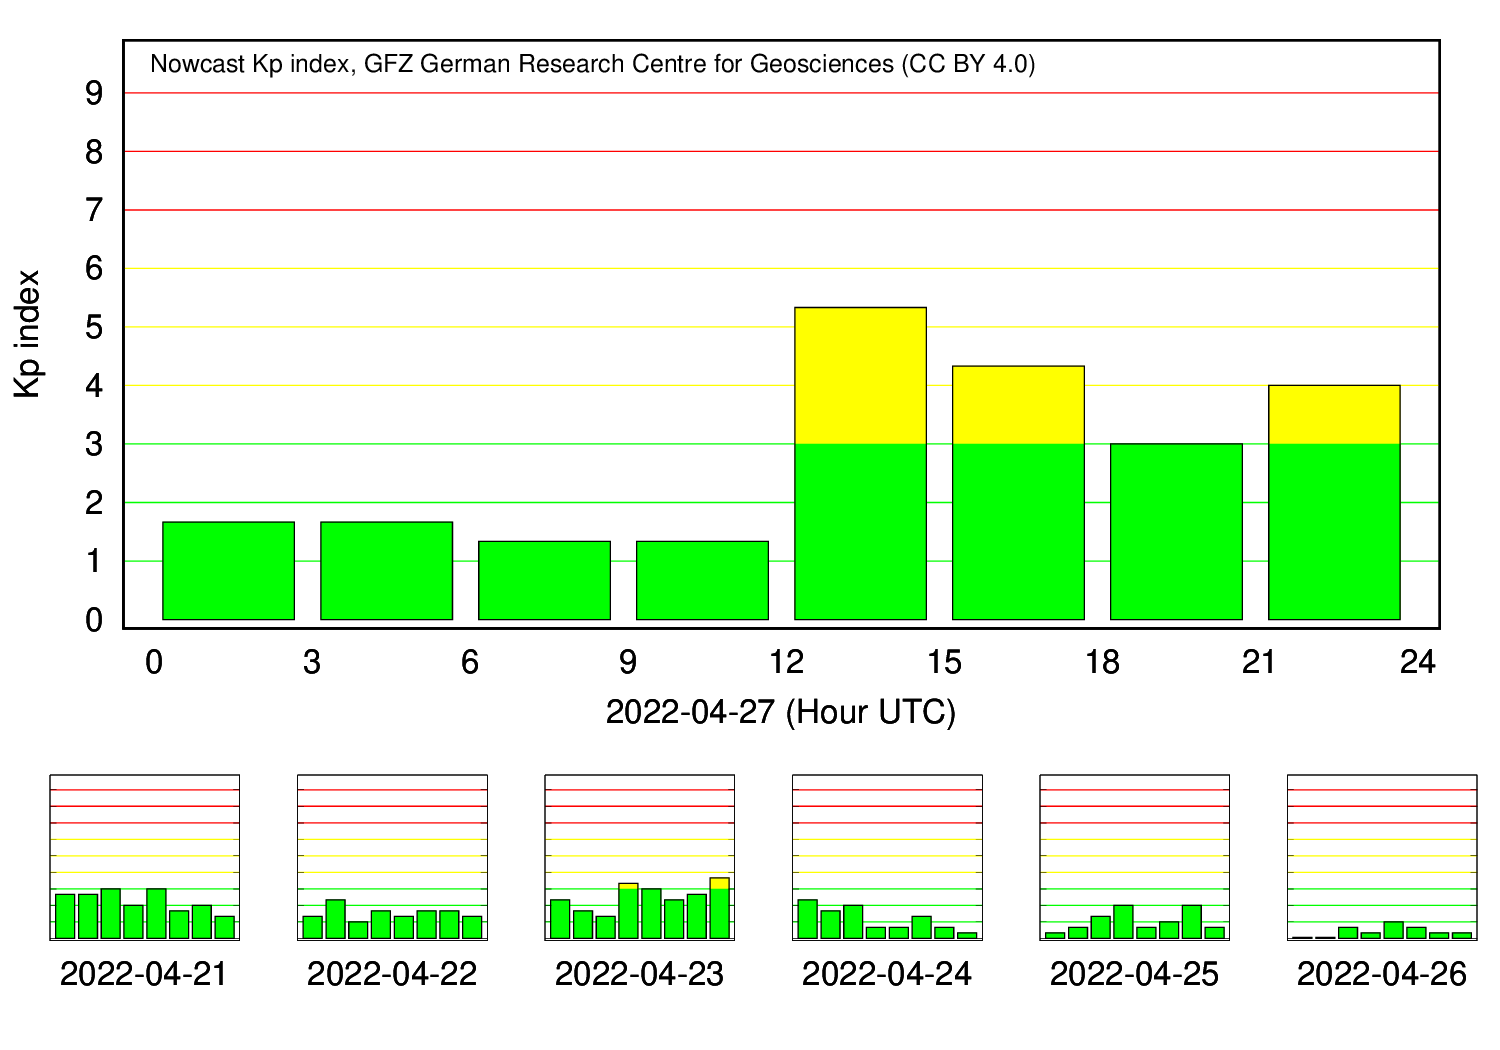
\includegraphics[width=14cm]{./figures//figureGeomag_6.png}

                        \end{figure}

                     \begin{figure}[H]
    
                        \centering
   
                             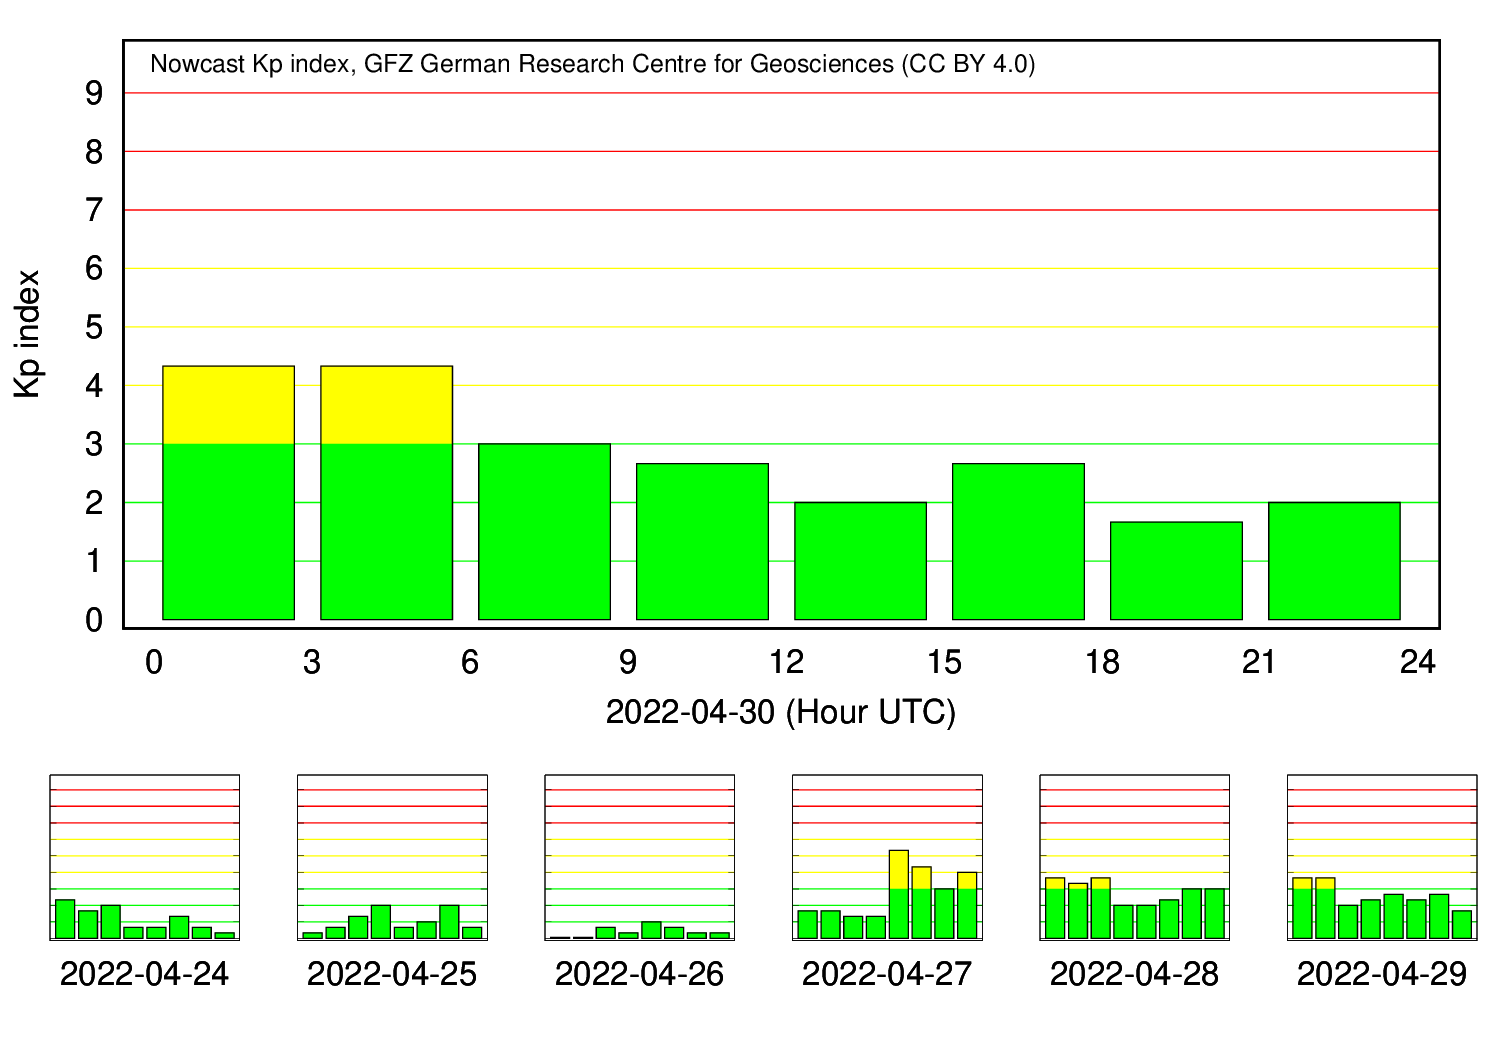
\includegraphics[width=14cm]{./figures//figureGeomag_7.png}

                        \end{figure}

                     \begin{figure}[H]
    
                        \centering
   
                             \includegraphics[width=14cm]{./figures//figureGeomag_8.png}

                        \end{figure}

                     \begin{itemize} 
\item Na semana de10 a 16/05, destacam-se os seguintes eventos relacionados a atividade geomagnética:
\item Os dados provenientes da rede de magnetômetros Embrace apresentaram instabilidades durante todo o período, com alguns eventos em destaque:
\item As maiores perturbações na componente H foram registradas nos dias 11, 13, e 14 de maio
\item A atividade geomagnética foi instável durante todo o índice AE, com o índice Dst oscilando em torno de zero. O Kp mais alto da semana foi de 3+
\item  A atividade auroral foi levemente intensificada nos dias 13, 14 e 15/05.
\item Campo magnético medido na órbita do satélite GOES apresentoualgumas instabilidades
\end{itemize} 
\section{Ionosfera} 
 \subsection{Responsável: Laysa Resende} 
 
\textbf{Boa Vista: }

 \begin{itemize}
\item Ocorreu spread-F todos os dias.
\item As camadas Es atingiu a escala 3 nos dias 12 e 13.
\item Ocorreu Blackout parcial no dia 10.
\end{itemize}
\begin{figure}[H]
    \centering
    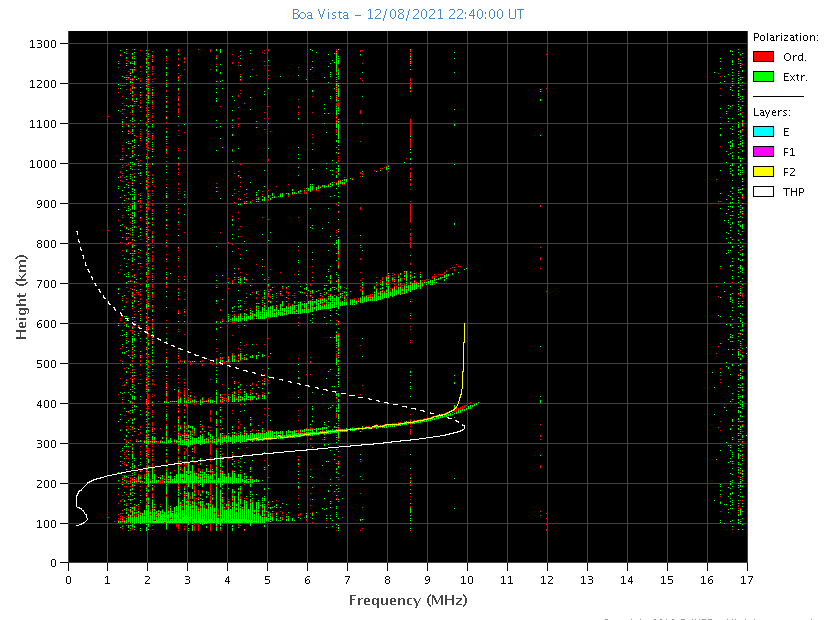
\includegraphics[width=14cm]{./figures//BoaVista.png}
\end{figure}

\textbf{Cachoeira Paulista:}

 \begin{itemize}
\item Ocorreu spread-F no dia 12.
\item As camadas Es dessa região atingiu a escala 3 nos dias 09 e 12.  
\end{itemize}
\begin{figure}[H]
    \centering
    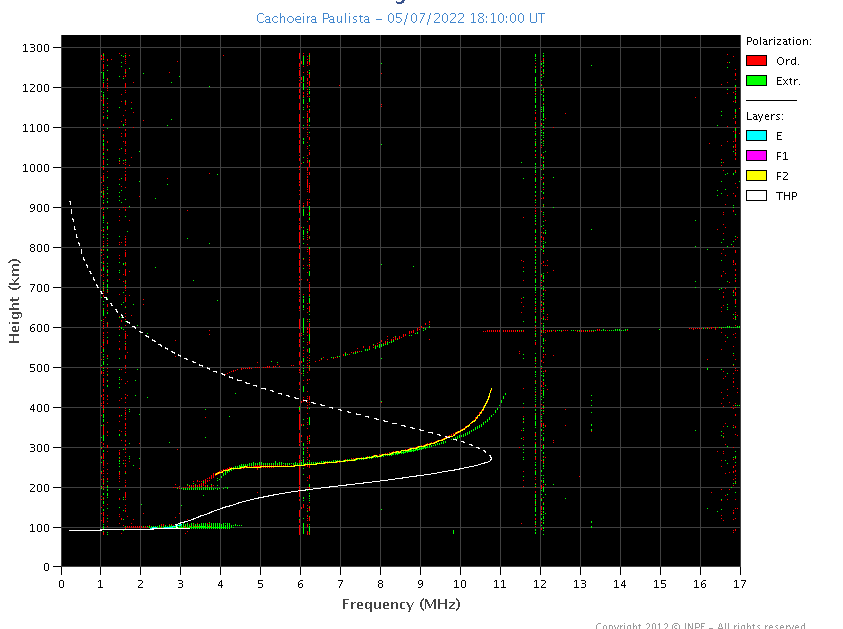
\includegraphics[width=14cm]{./figures//CachoeiraPaulista.png}
\end{figure}

\textbf{São Luís: }

 \begin{itemize}
\item Ocorreu spread -F durante toda a semana. 
\item As camadas Es dessa região atingiu a escala 5 no dia 11. 
\item Ocorreu Blackout parcial no dia 10.
\end{itemize}
\begin{figure}[H]
    \centering
    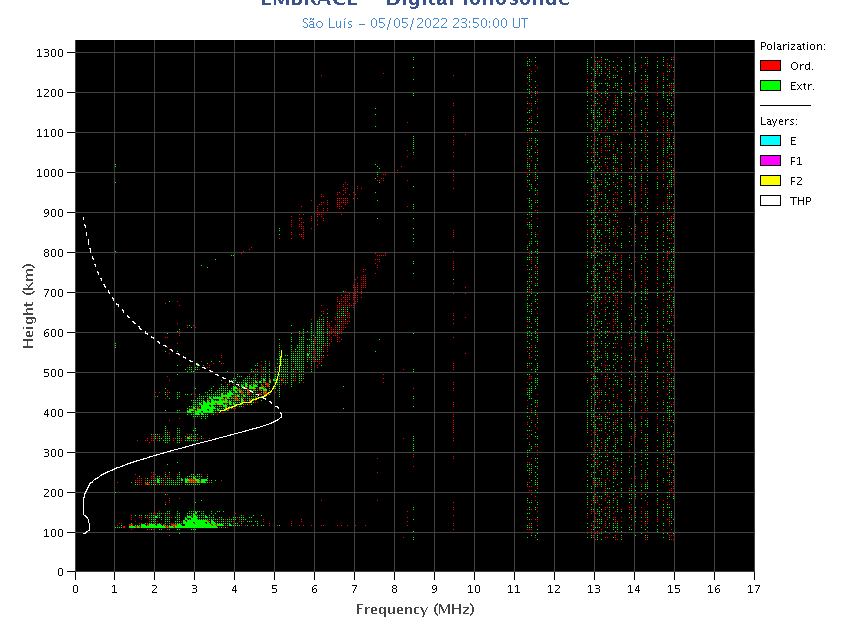
\includegraphics[width=14cm]{./figures//SãoLuís.png}
\end{figure}

\section{Cintilação} 
 \subsection{Responsável: Siomel Savio Odriozola} 
 
Neste reporte sobre o índice de cintilação S4, foram apresentados dados das 
estações SLMA em São Luiz/MA, STSN em Sinop/MG, UFBA em Bahía/BA e 
SJCE em São José dos Campos/SP. O índice S4 acompanha a presença de 
irregularidades na ionosfera quando elas têm uma escala espacial ~ 360 m.  
As quatro estações analisadas não apresentaram valores relevantes do índice 
S4 durante toda a semana. A Figura 1 mostra os valores para as estações SLMA 
(painel superior) e SJCE(painel inferior) 

    \begin{figure}[H]
        \centering
        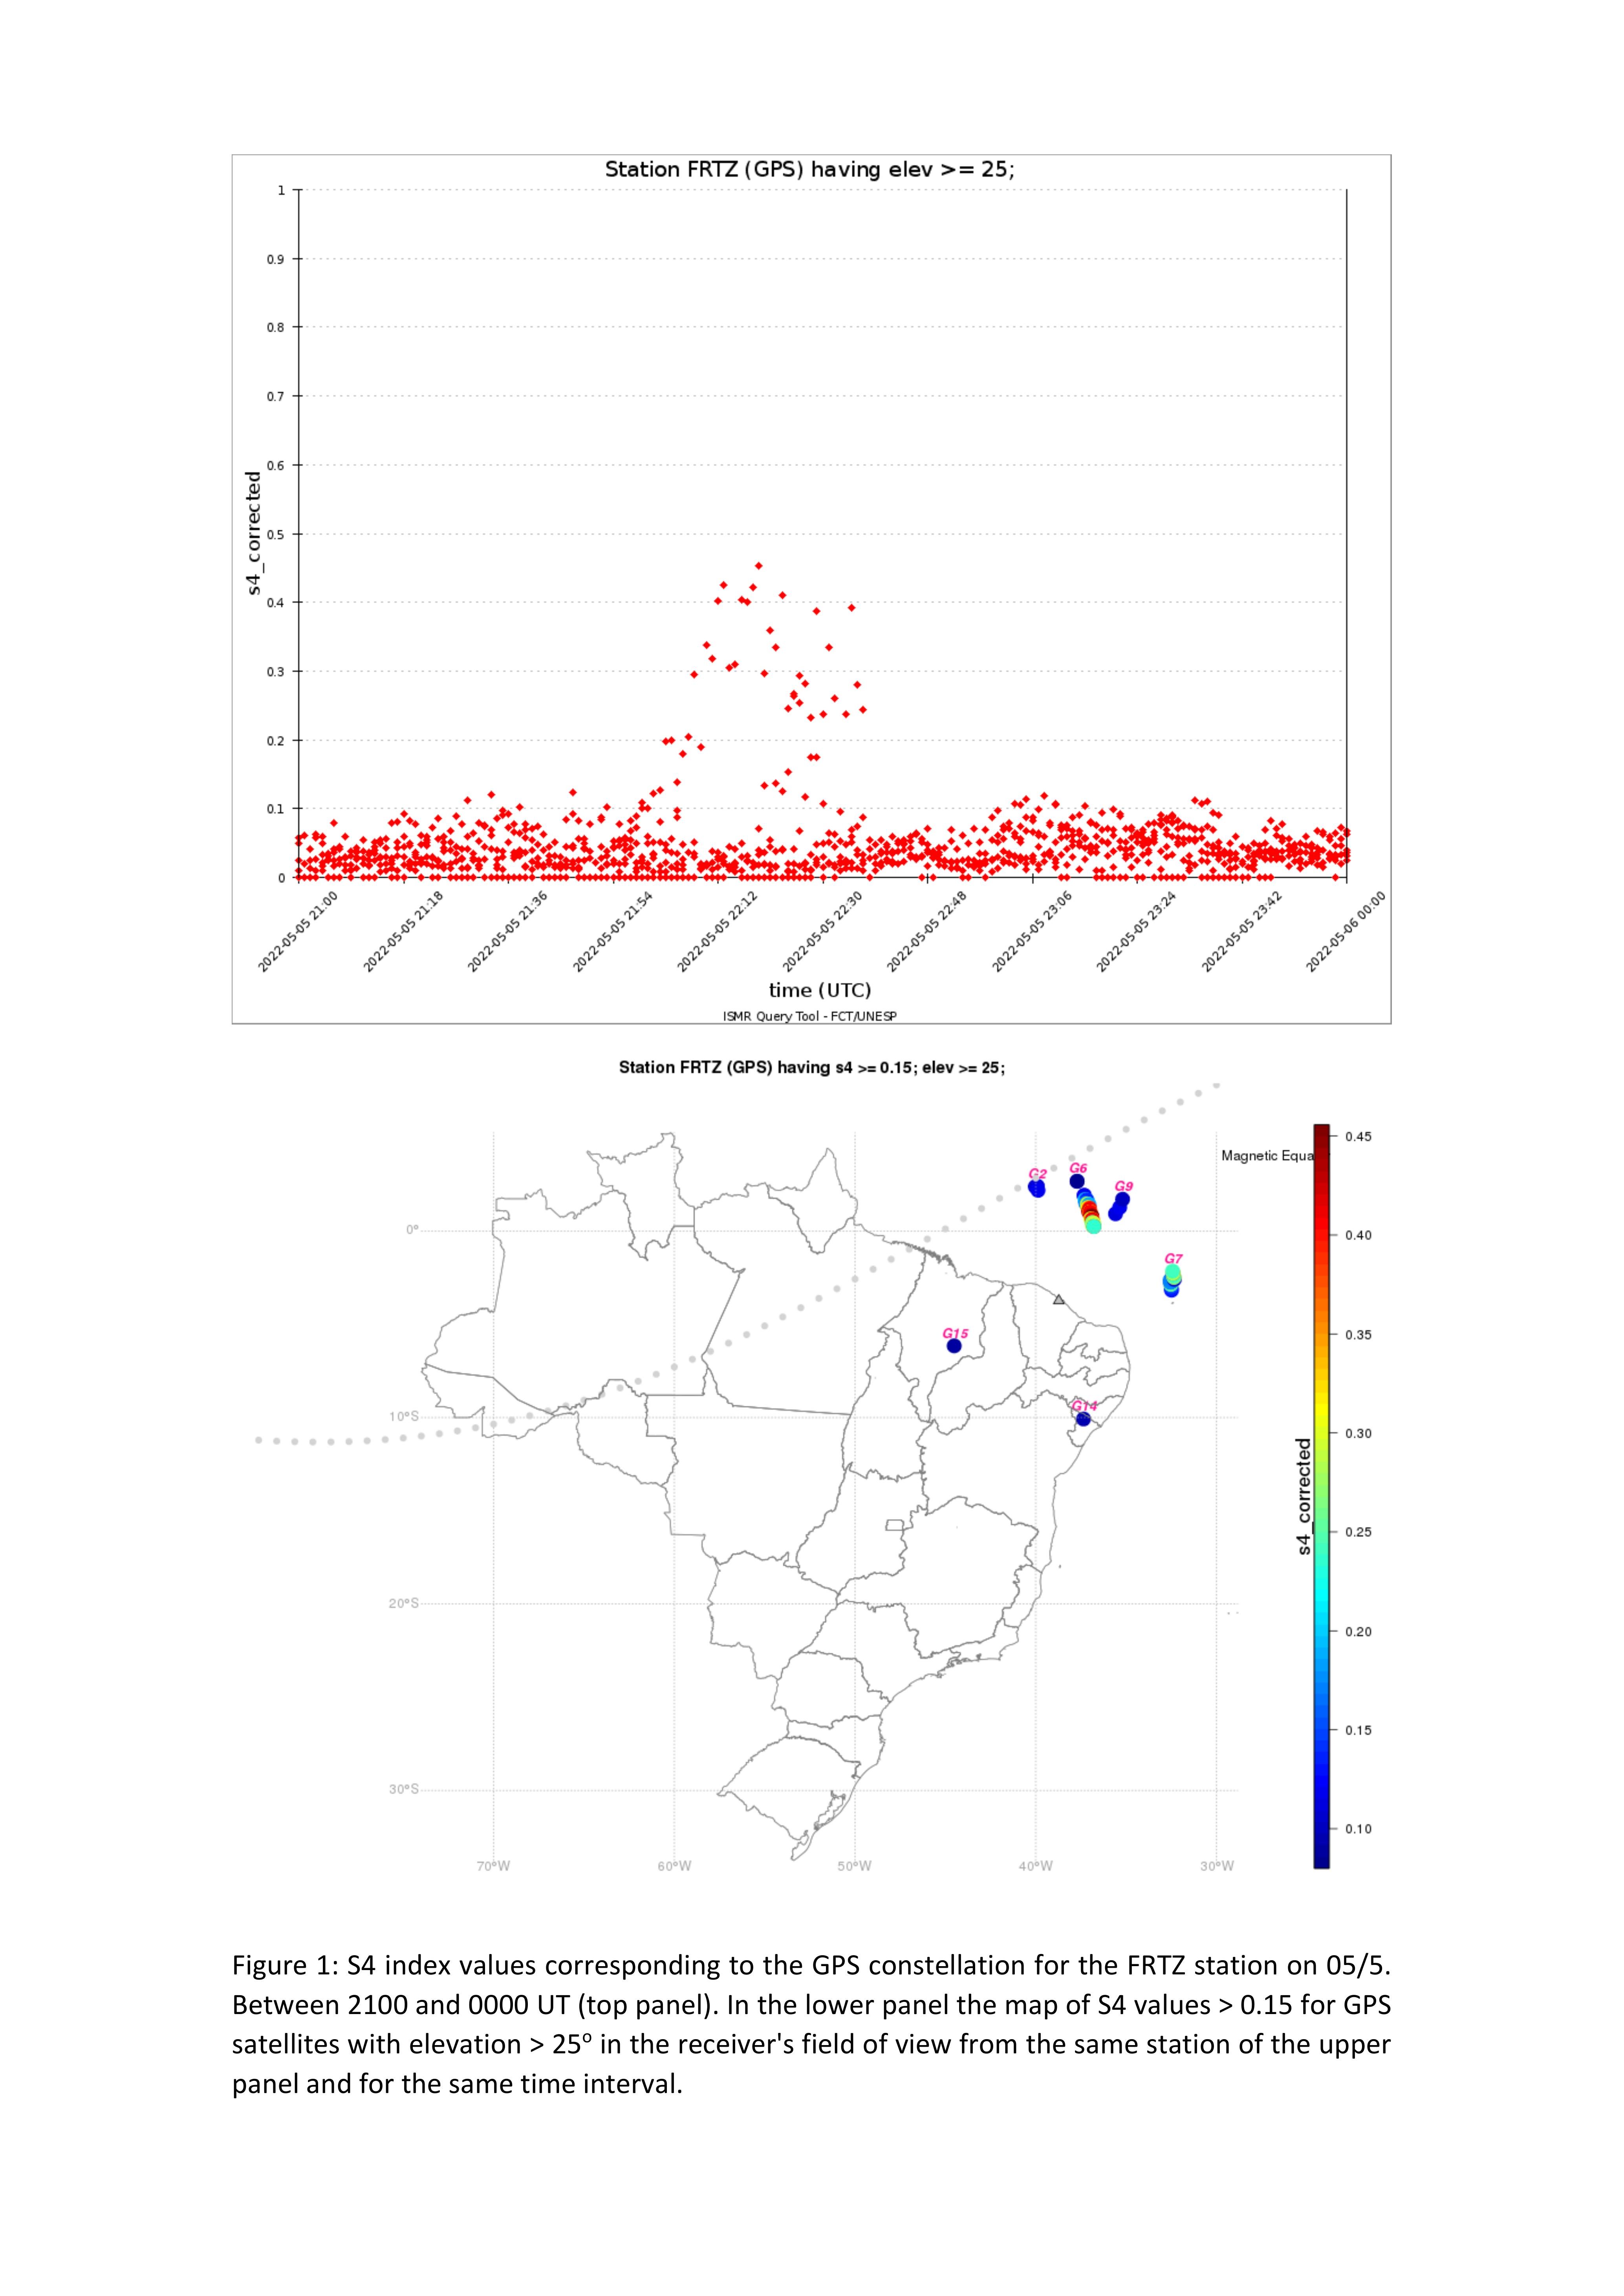
\includegraphics[width=14cm]{./figures/pt_outfileScint_0.jpg}
    \end{figure} 
 

    \section{Imageador All-Sky} 
 \subsection{Responsável: LUME} 
 
\begin{figure}[H]
    
                        \centering
   
                             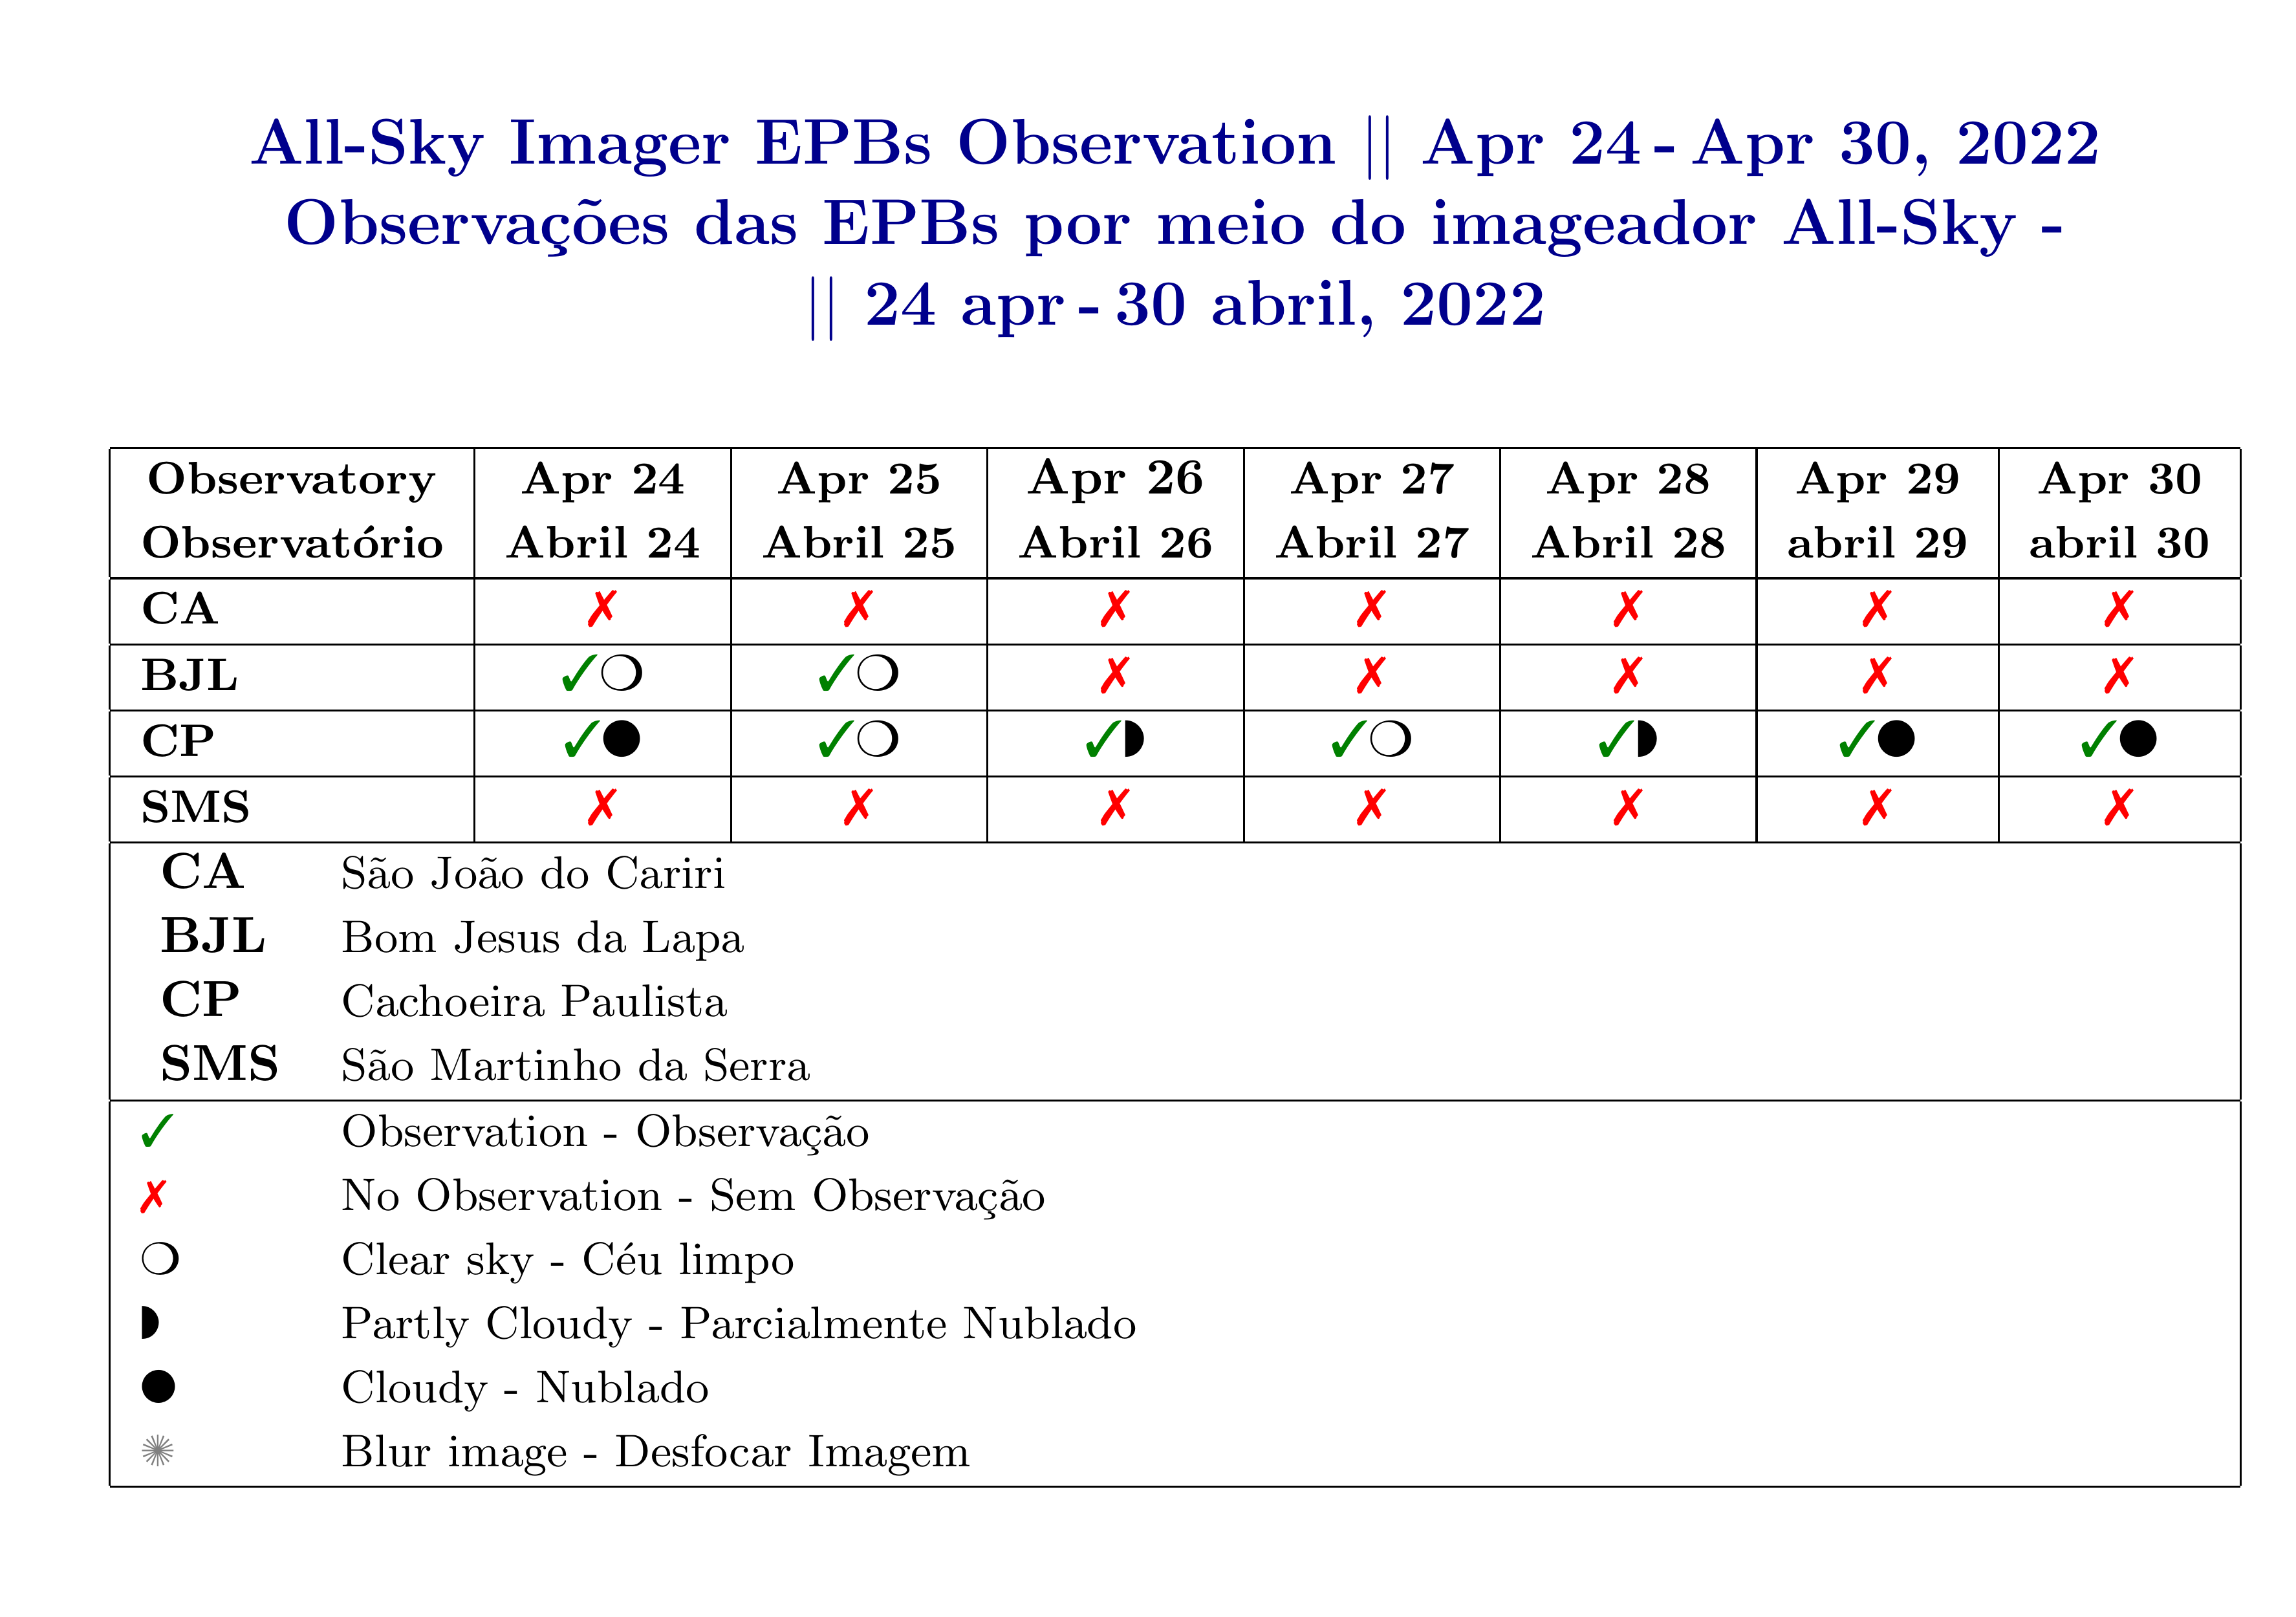
\includegraphics[width=14cm]{./figures//figureImager_0.png}

                        \end{figure}

                     \begin{itemize} 
 \item  No observatorio de Sao Joao do Cariri, nao observa bolhas de plasma durante todo o perıodo. 
\item  No observatorio de Bom de Jesus da Lapa, nao houve observacao devido a problemas tecnicos. 
\item  No observatorio de Cachoeira Paulista, nao foi observado bolhas de plasma durante o perıodo. 
\item  Por fim, no observatorio de Sao Martinho da Serra, nao foi observado bolhas durante a semana. 
\end{itemize} 
 TEC 
\begin{itemize} 
 \item  Nao foi observado bolhas de plasma durante todo o perıodo. Como a sazon- alidade de bolhas esta no fim, as bolhas apresentam dimensoes espaciais pequenas e ficam difıceis de observar no mapas de TEC. 
\end{itemize} 
 

\end{document}